%% The following is a directive for TeXShop to indicate the main file
%%!TEX root = diss.tex
\chapter{Supporting Materials}

% This would be any supporting material not central to the dissertation.
% For example:
% \begin{itemize}
% \item radiometry
% \item technical details of MVS, PS, SL, SfS, etc
% \end{itemize}

\section{Material of real-world objects}
\label{sec:real_world_dataset}
\begin{table}[!hbtp]
  \centering
  \begin{tabular}{*{9}{c}}
  \multicolumn{3}{l}{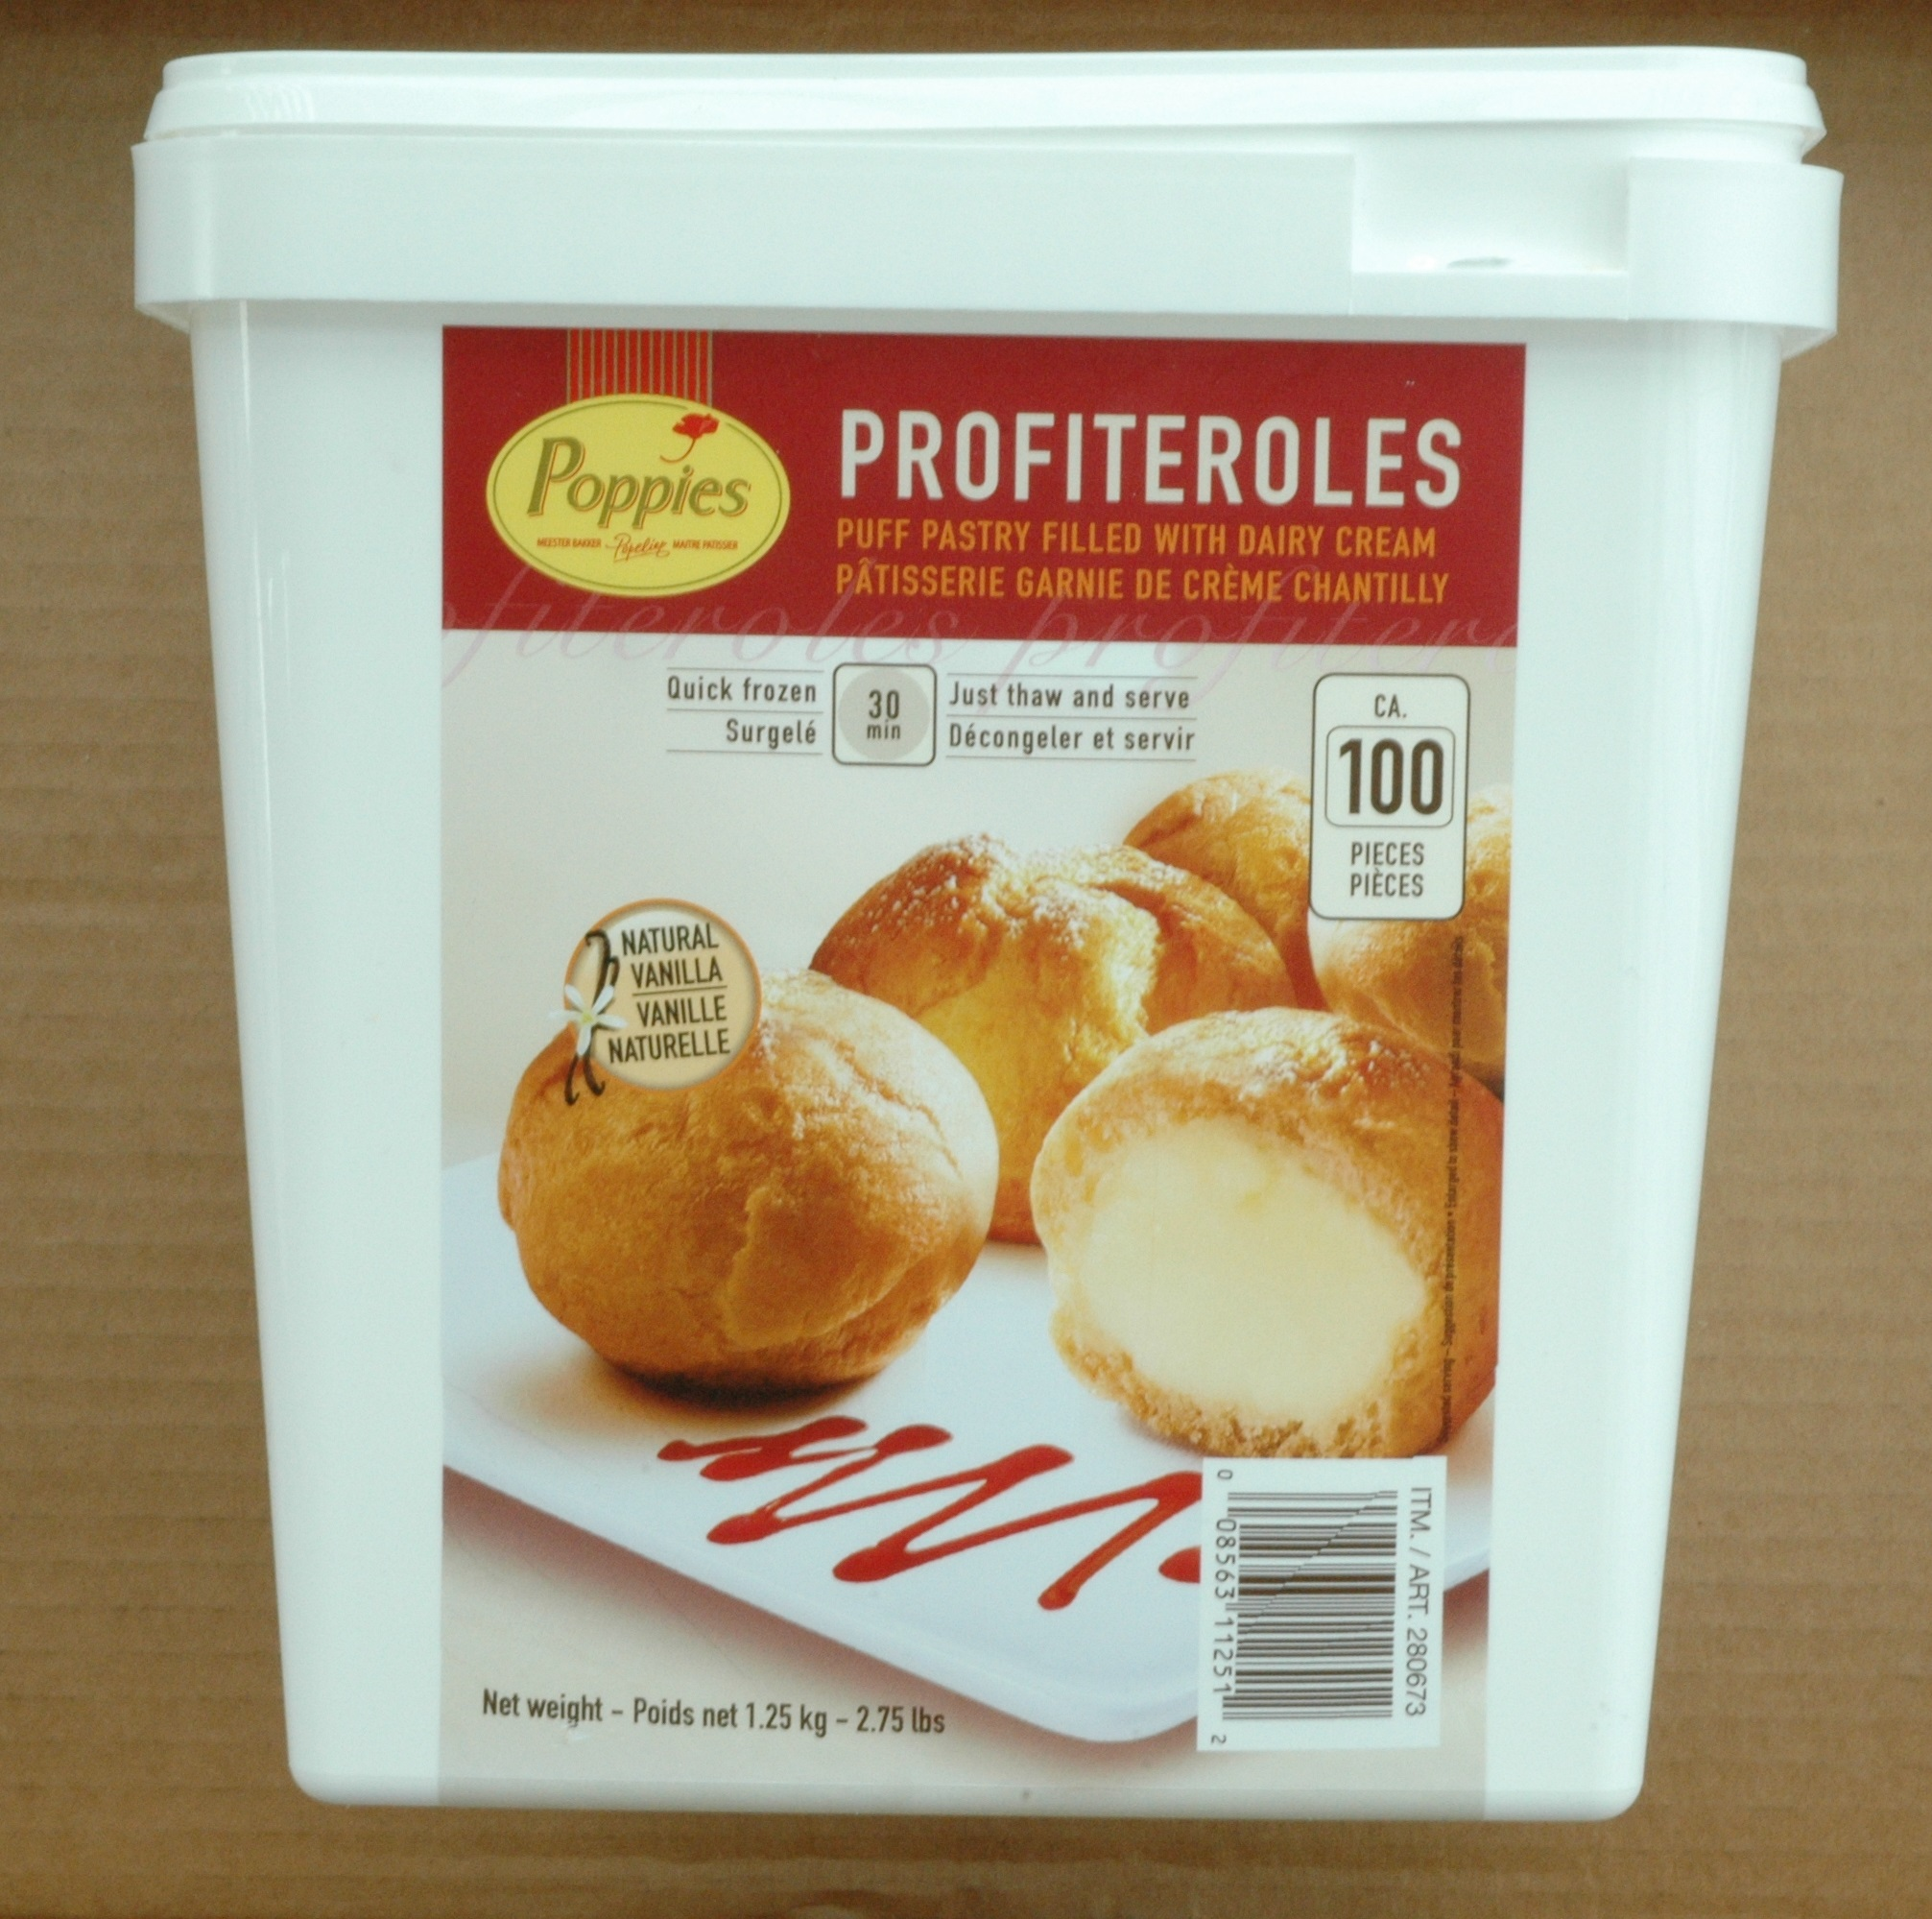
\includegraphics[width=0.33\textwidth]{interp/real_world_img/box/box}} &
  \multicolumn{3}{l}{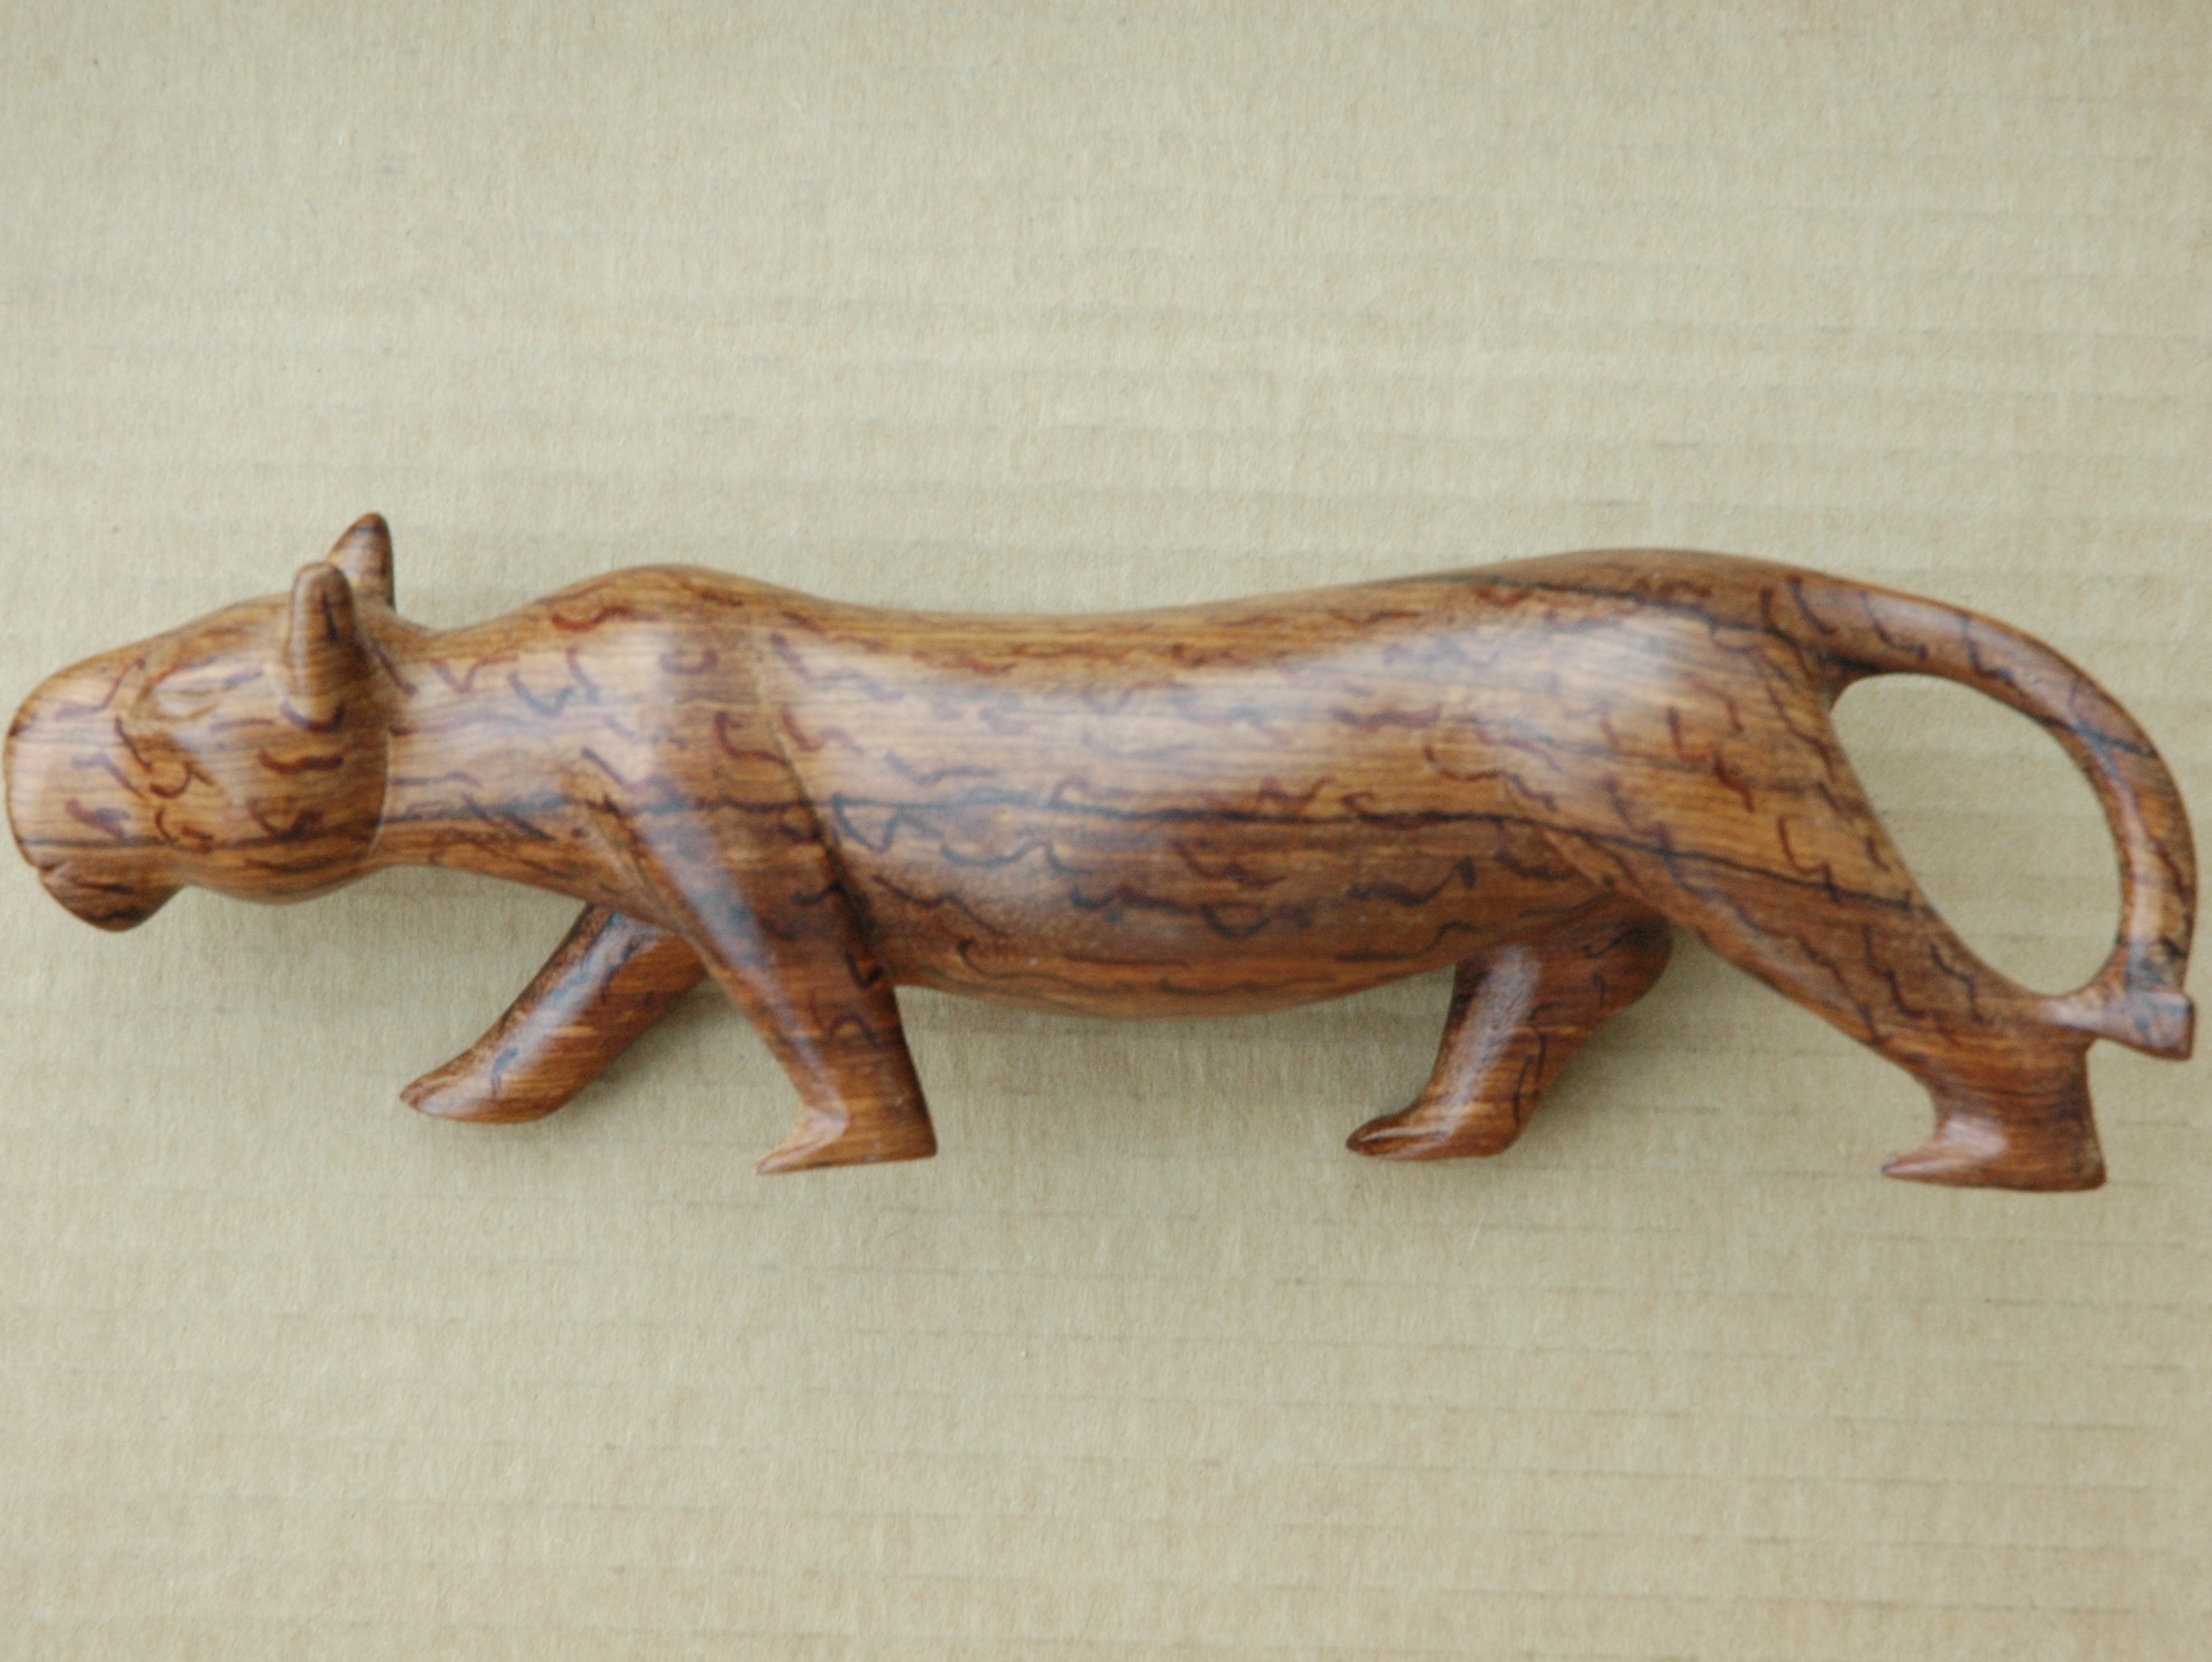
\includegraphics[width=0.33\textwidth]{interp/real_world_img/cat0/cat0}} &
  \multicolumn{3}{l}{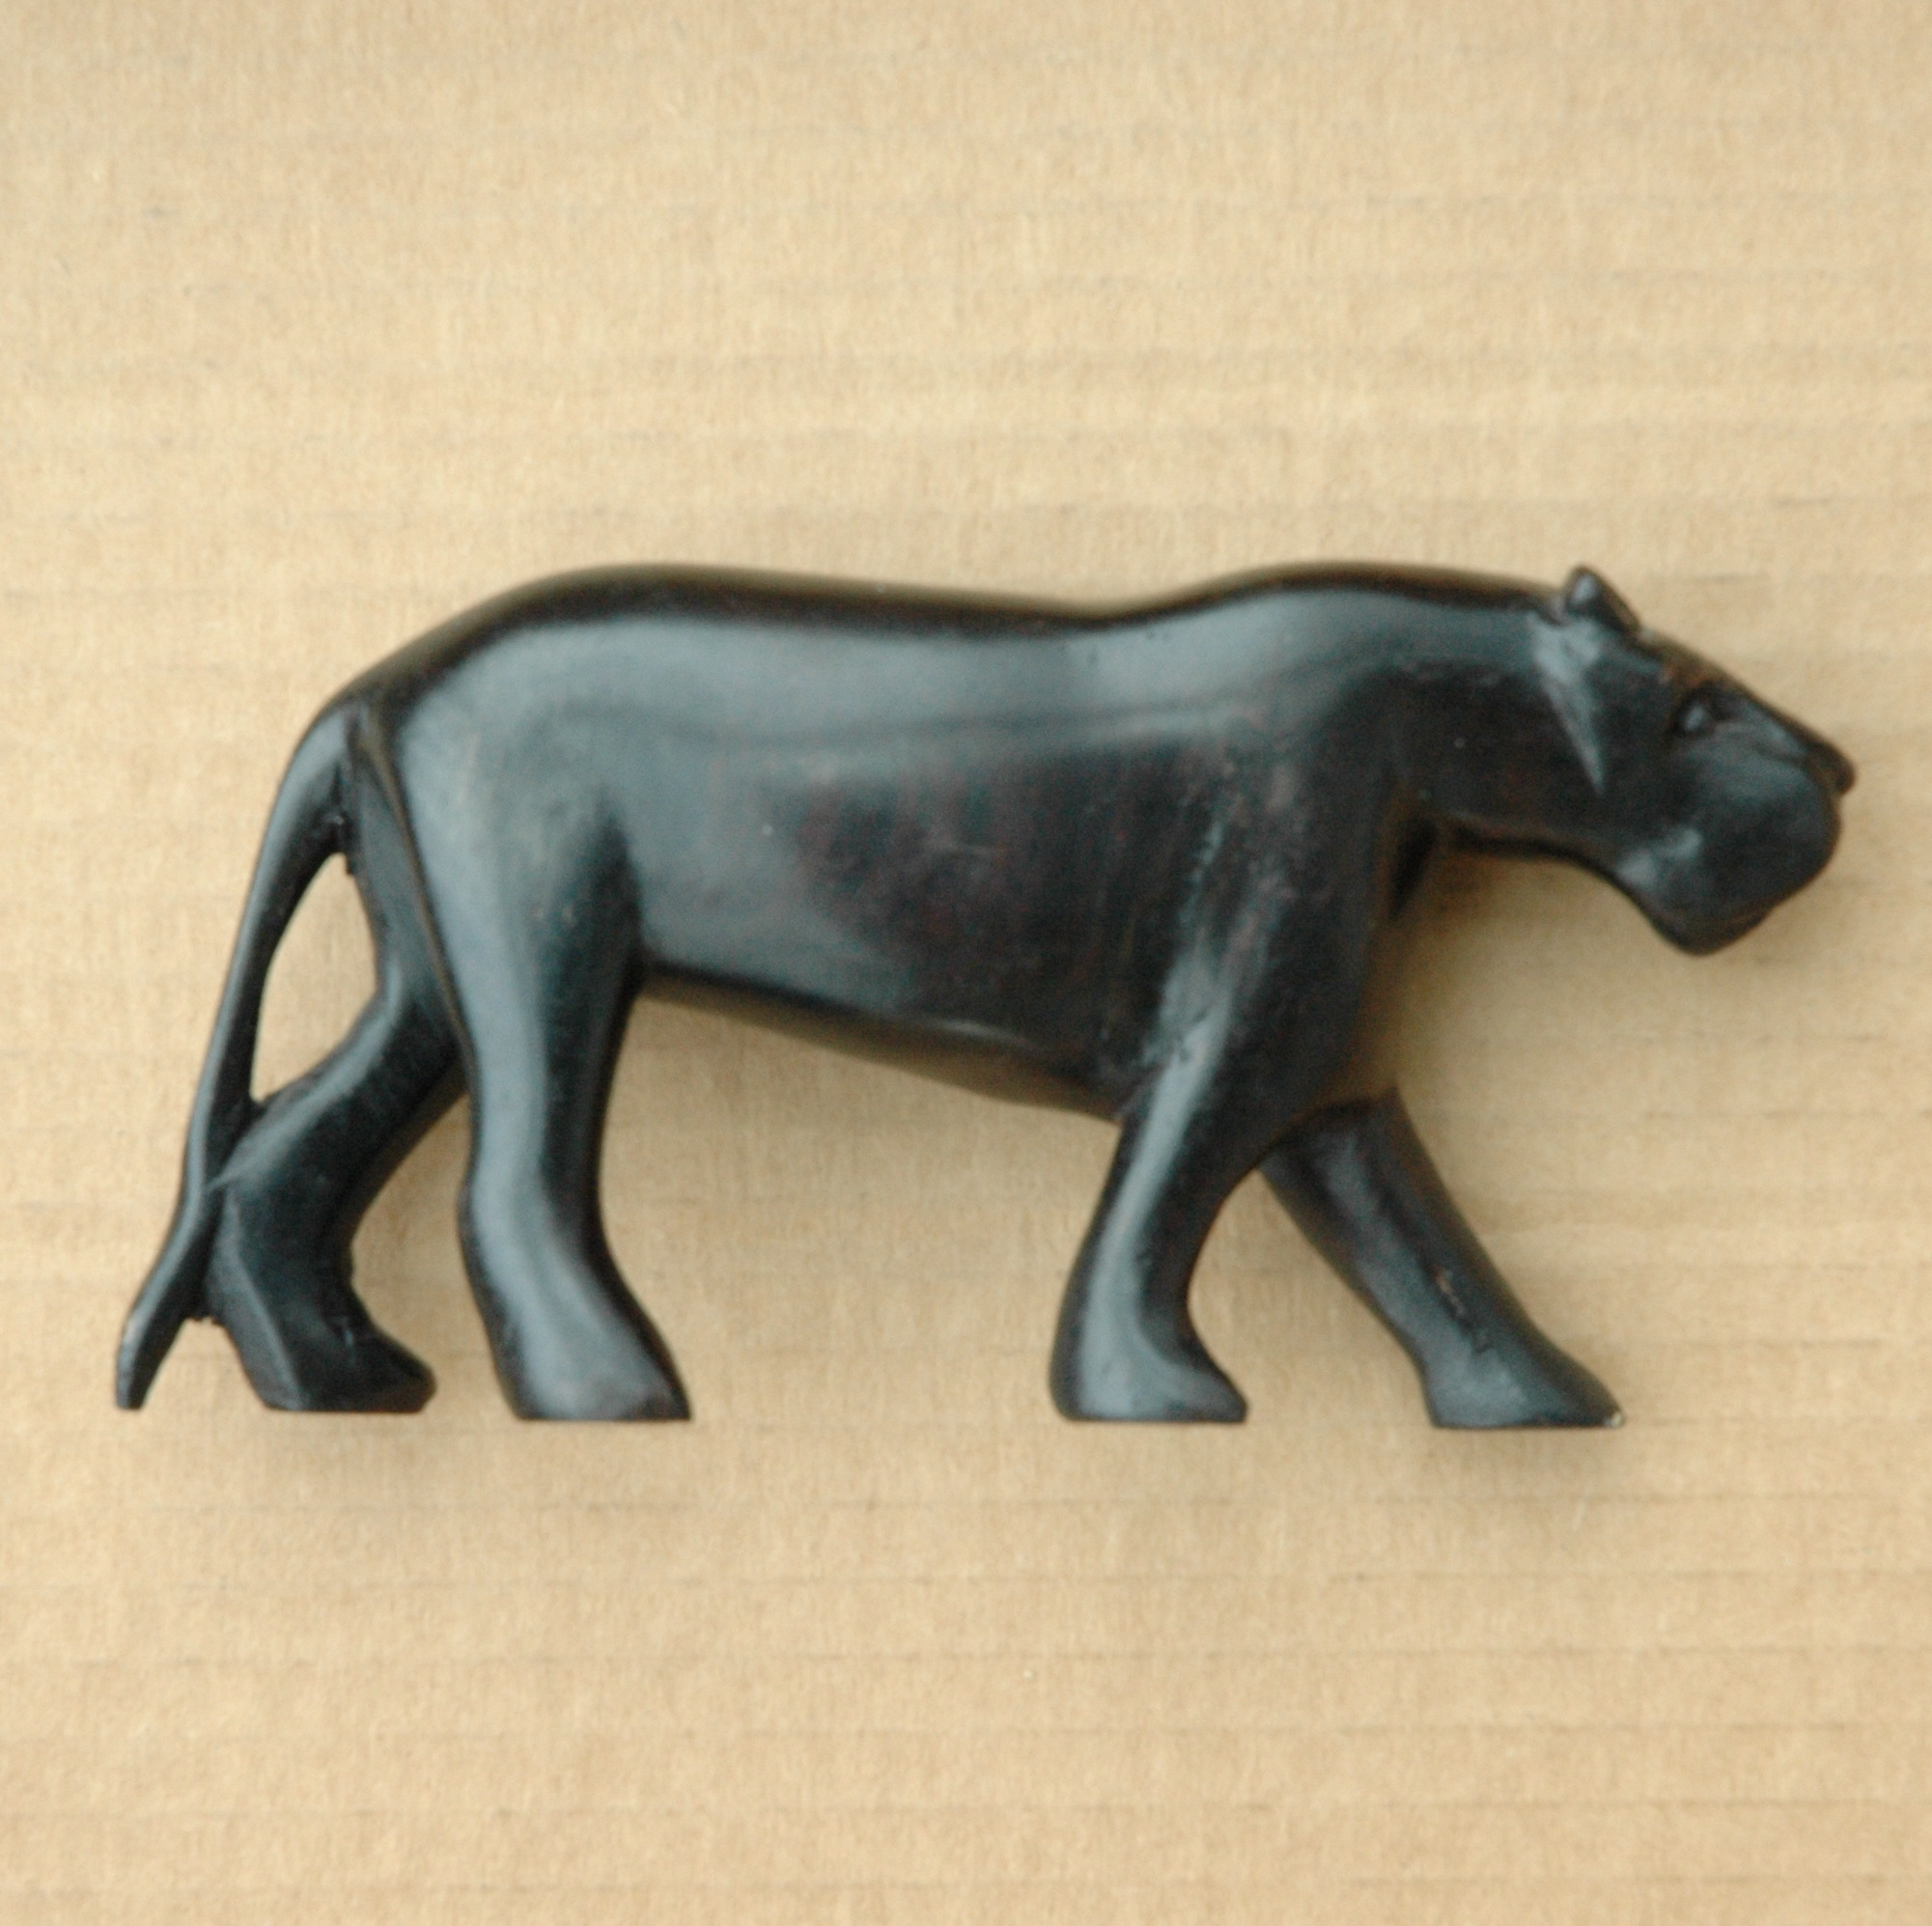
\includegraphics[width=0.33\textwidth]{interp/real_world_img/cat1/cat1}}\\
  % \includegraphics[width=0.1\textwidth]{interp/real_world_img/box/base_00} &
  % \includegraphics[width=0.1\textwidth]{interp/real_world_img/box/base_01} & 
  % \includegraphics[width=0.1\textwidth]{interp/real_world_img/box/base_02} &
  % \includegraphics[width=0.1\textwidth]{interp/real_world_img/cat0/base_00} & 
  % \includegraphics[width=0.1\textwidth]{interp/real_world_img/cat0/base_01}& &
  % \includegraphics[width=0.1\textwidth]{interp/real_world_img/cat1/base_00} &\\
  \multicolumn{3}{c}{(a). box} & \multicolumn{3}{c}{(b). cat0} & \multicolumn{3}{c}{(c). cat1} \\
  \multicolumn{3}{l}{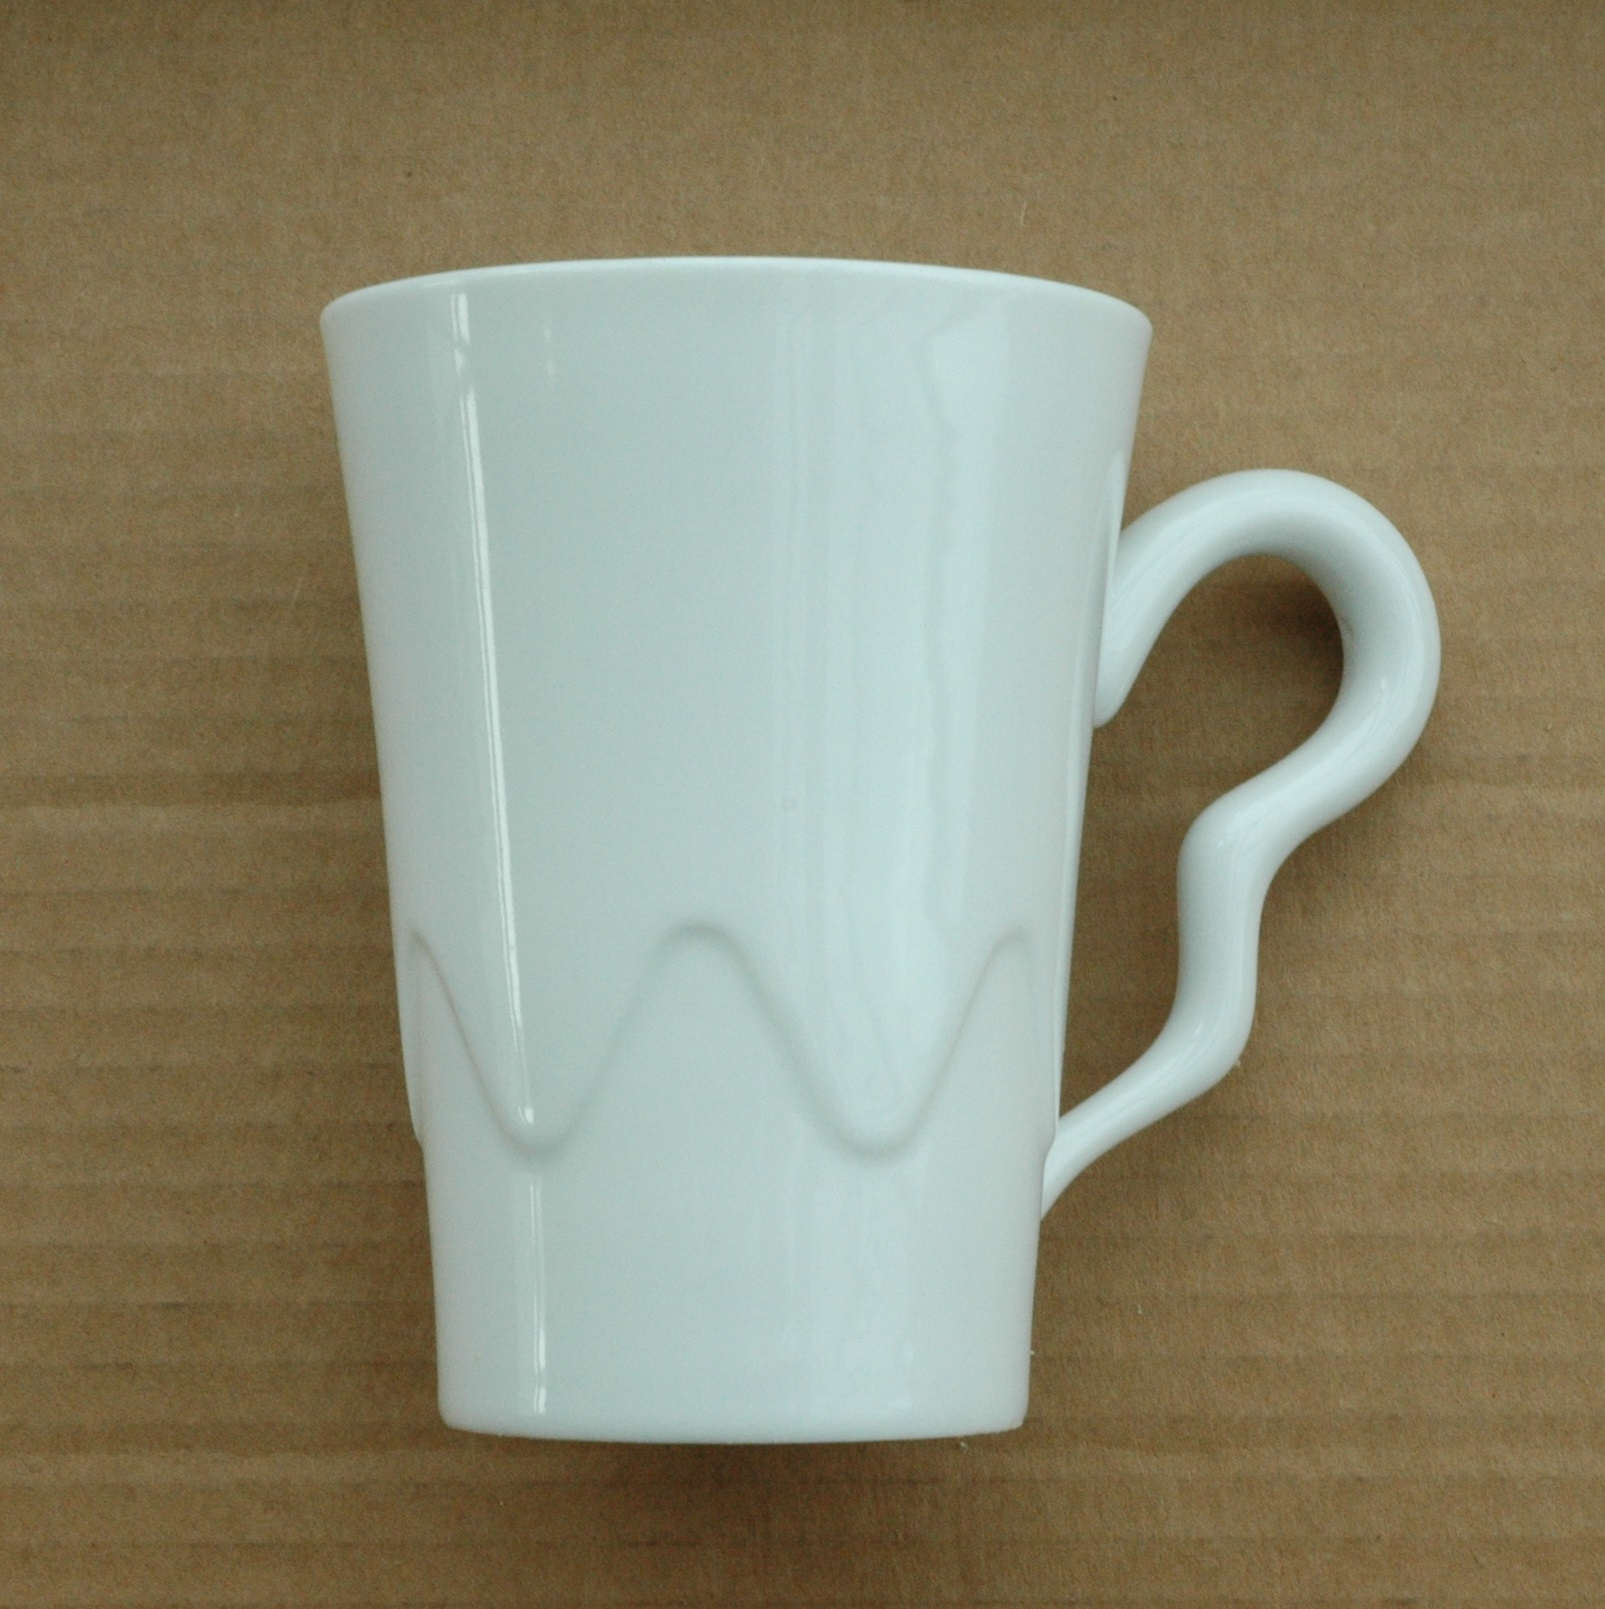
\includegraphics[width=0.33\textwidth]{interp/real_world_img/cup/cup}} &
  \multicolumn{3}{l}{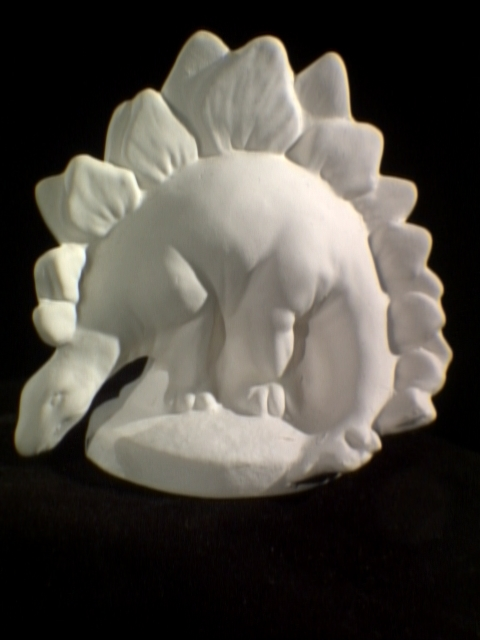
\includegraphics[width=0.33\textwidth]{interp/real_world_img/dino/dino}} &
  \multicolumn{3}{l}{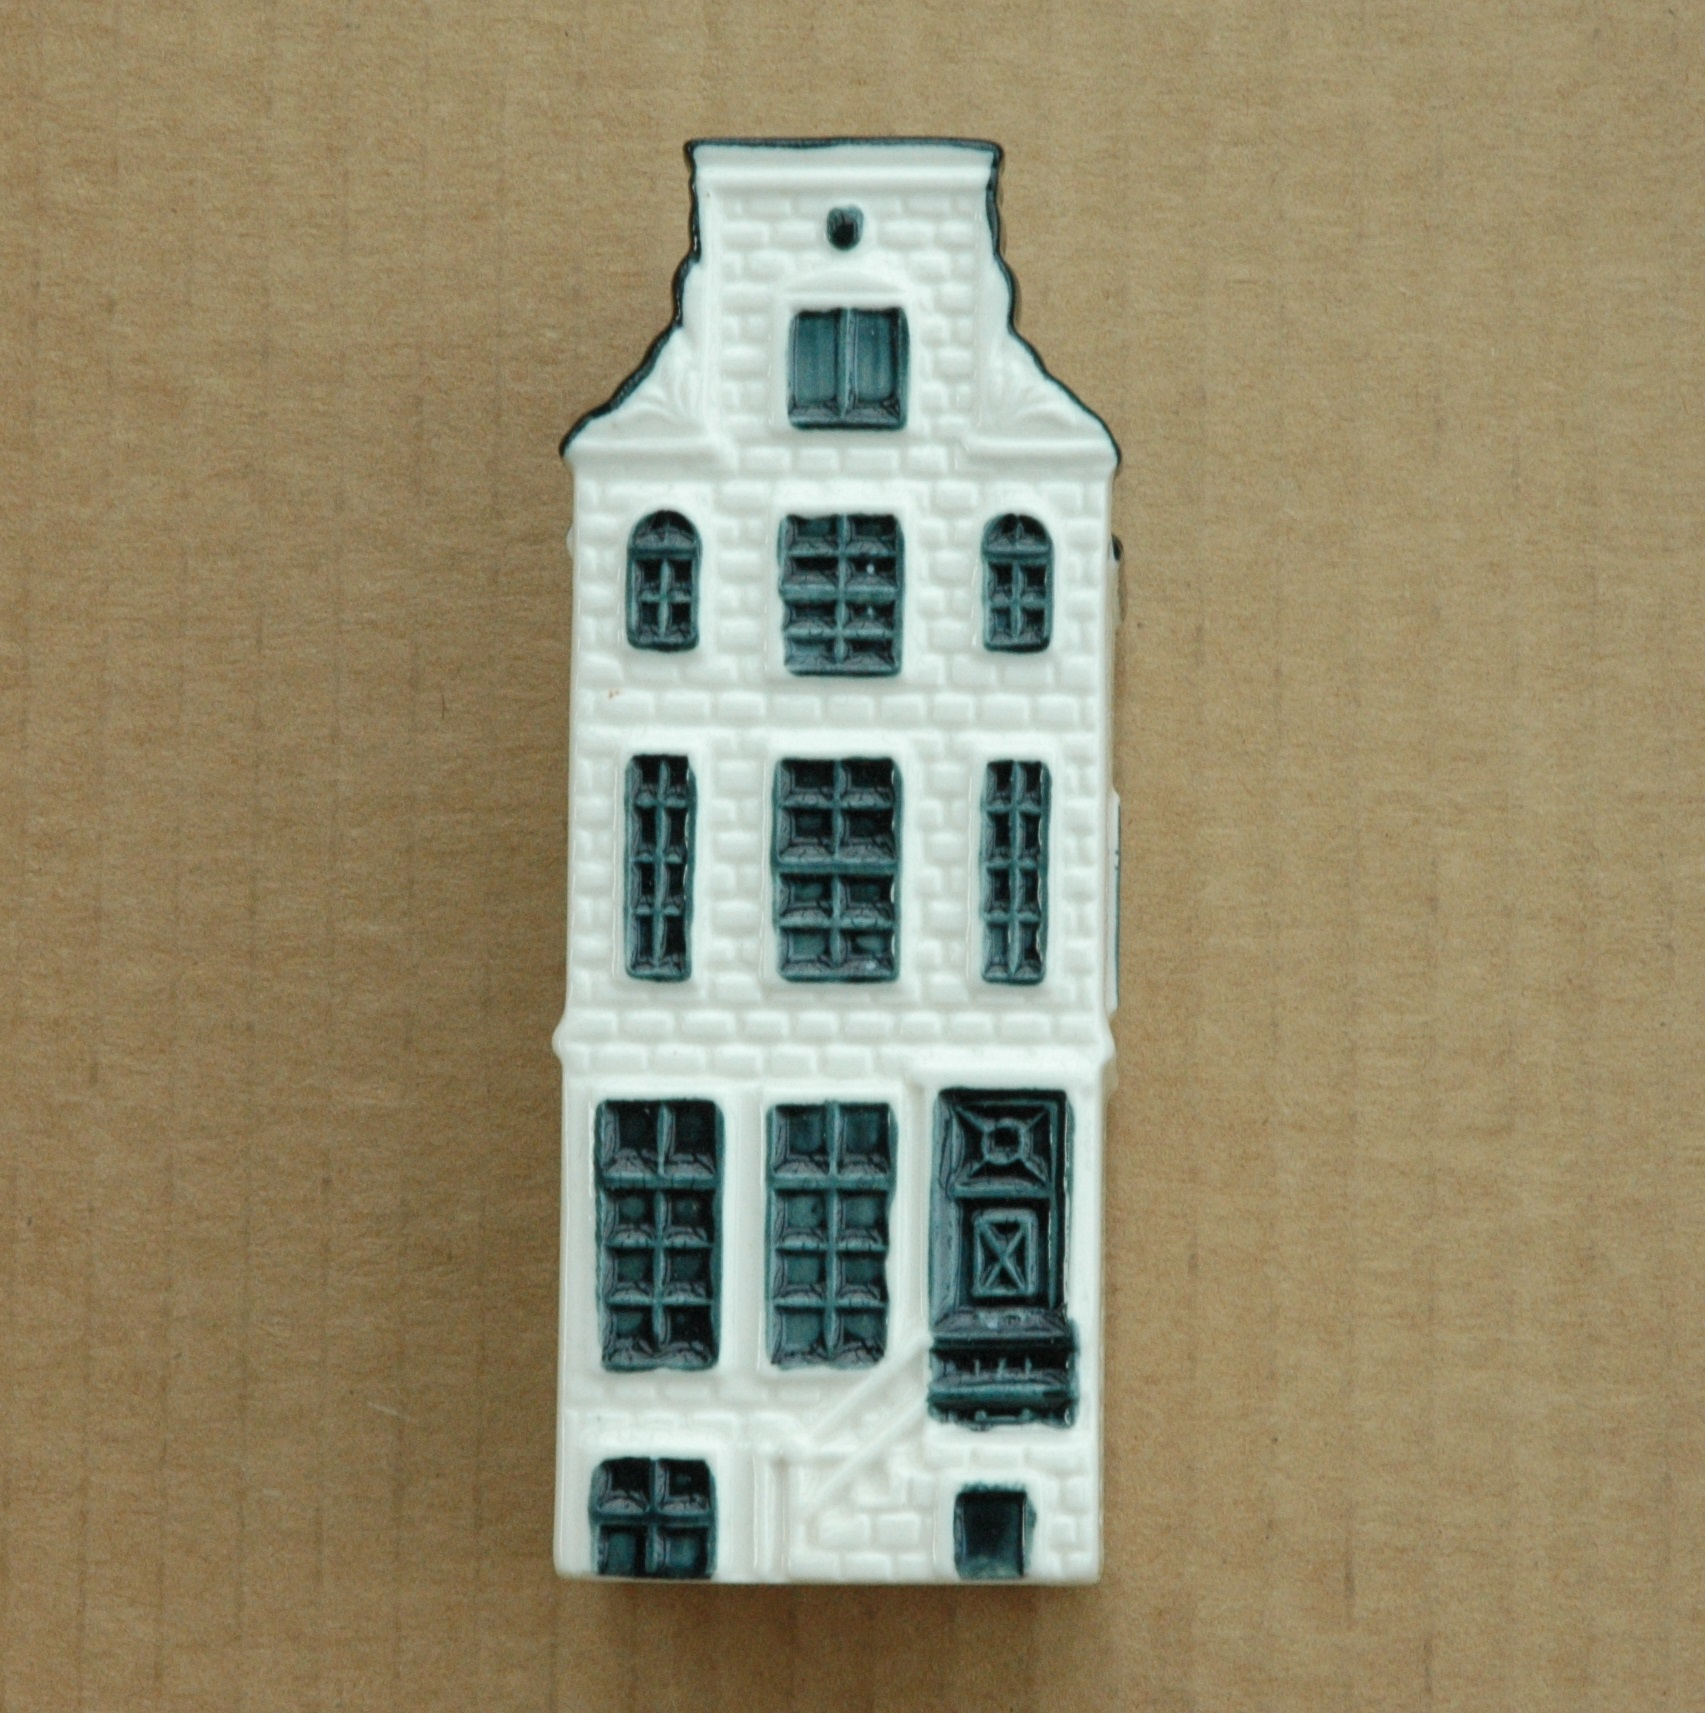
\includegraphics[width=0.33\textwidth]{interp/real_world_img/house/house}}\\
  % \includegraphics[width=0.1\textwidth]{interp/real_world_img/cup/base_00} & & &
  % \includegraphics[width=0.1\textwidth]{interp/real_world_img/dino/base_00} & 
  % \includegraphics[width=0.1\textwidth]{interp/real_world_img/dino/base_01} & 
  % \includegraphics[width=0.1\textwidth]{interp/real_world_img/dino/base_02} &
  % \includegraphics[width=0.1\textwidth]{interp/real_world_img/house/base_00} &
  % \includegraphics[width=0.1\textwidth]{interp/real_world_img/house/base_01} & \\
  \multicolumn{3}{c}{(d). cup} & \multicolumn{3}{c}{(e). dino} & \multicolumn{3}{c}{(f). house} \\
  \end{tabular}
  \caption{Images of the real-world objects.}
  \label{fig:real_data_material}
\end{table}

\begin{table}[!hbtp]
  \centering
  \begin{tabular}{*{9}{c}}
  \multicolumn{3}{l}{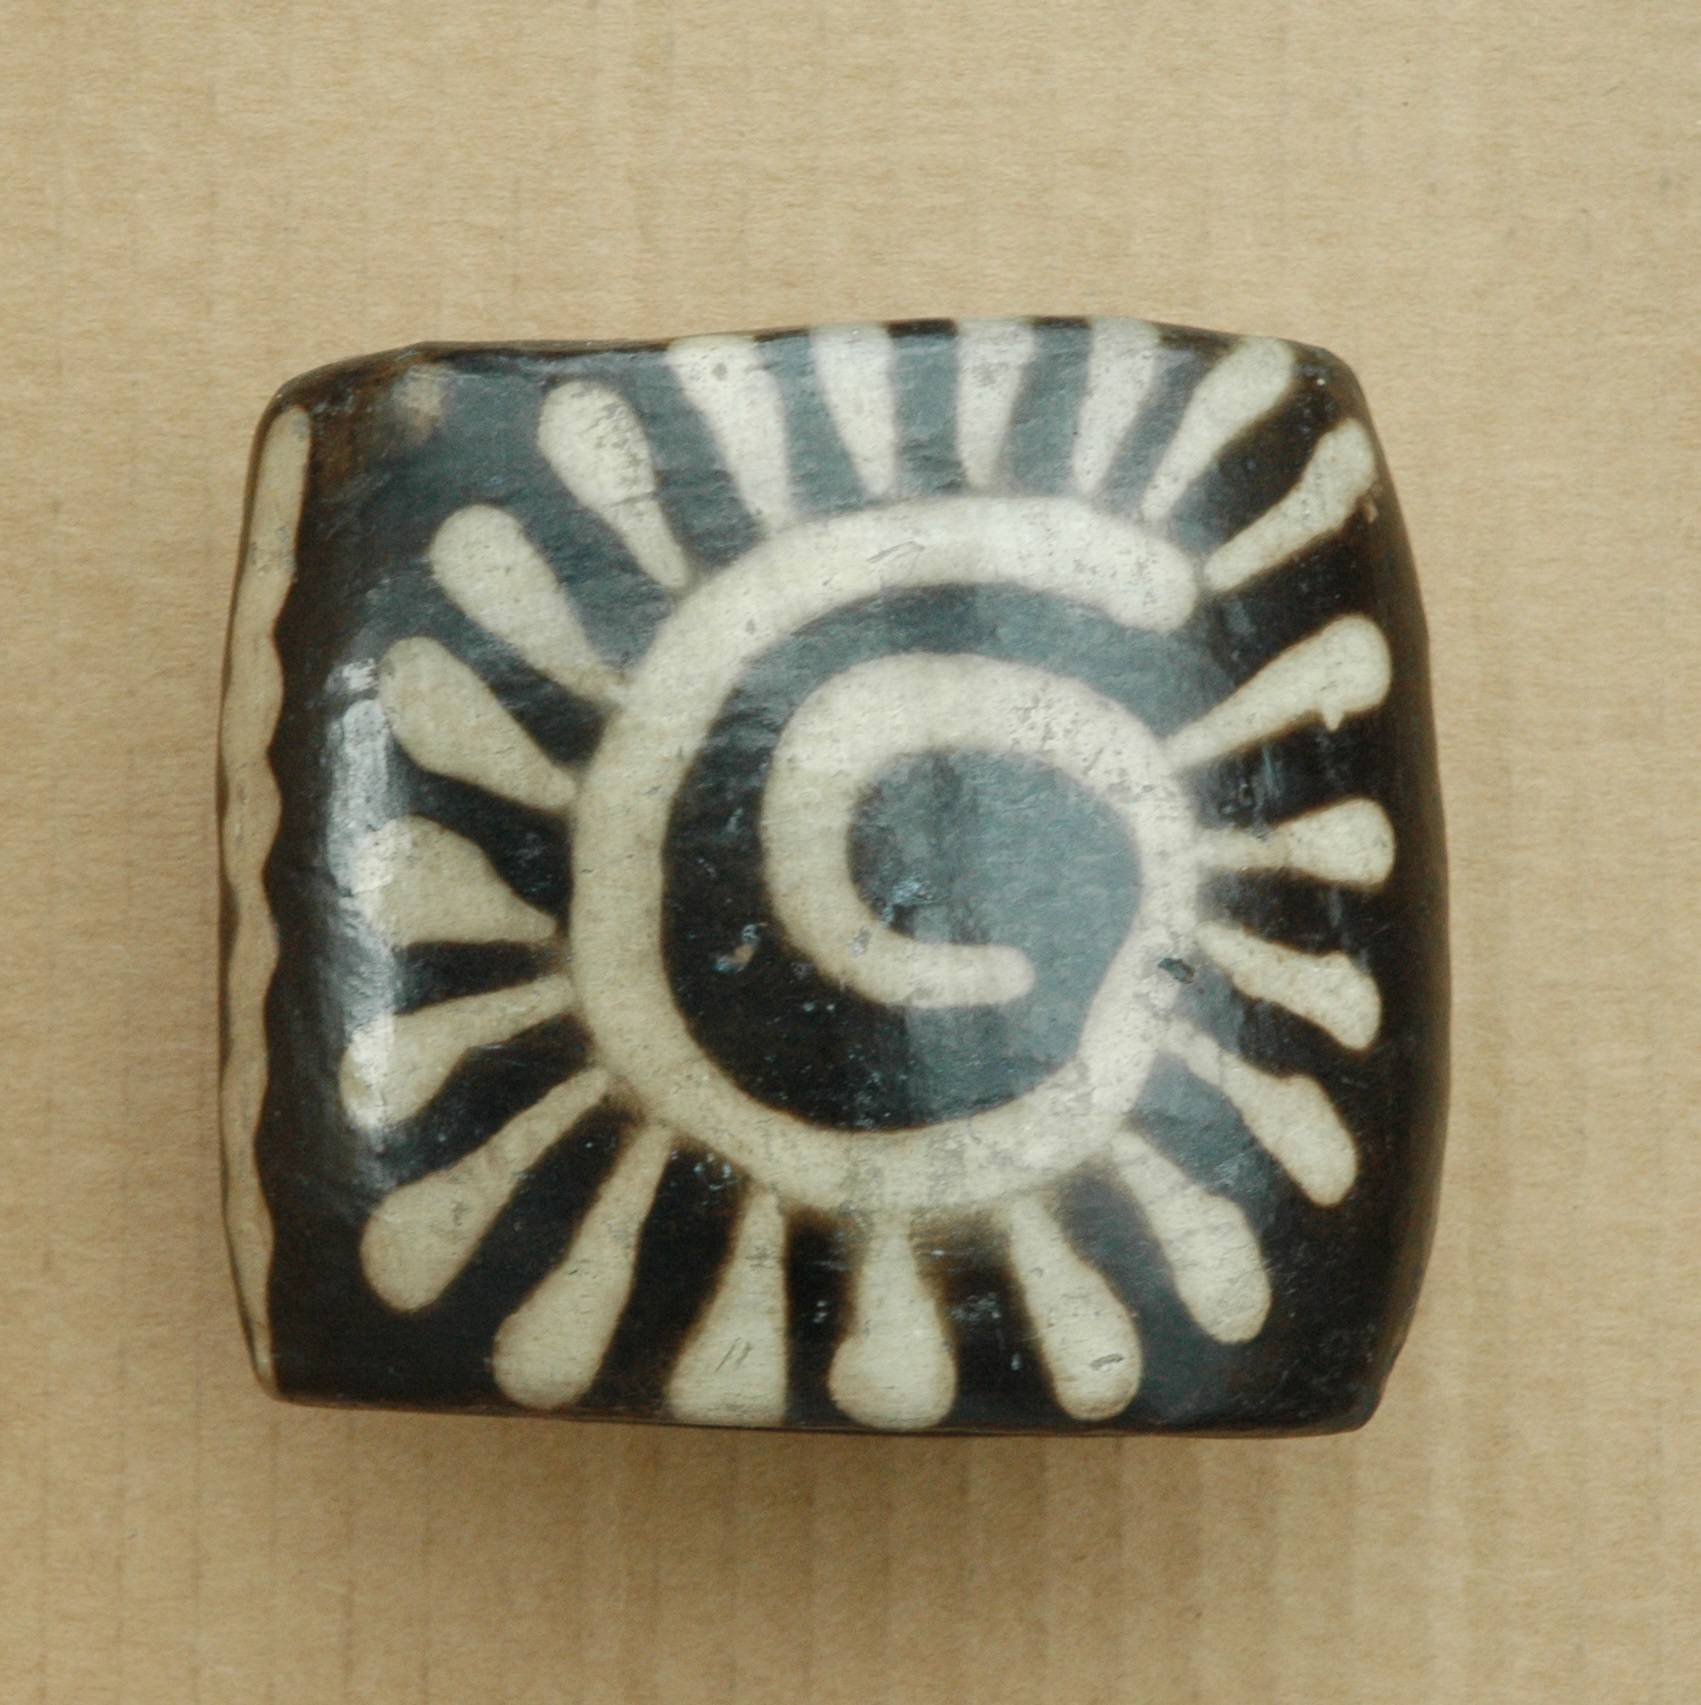
\includegraphics[width=0.33\textwidth]{interp/real_world_img/pot/pot}} &
  \multicolumn{3}{l}{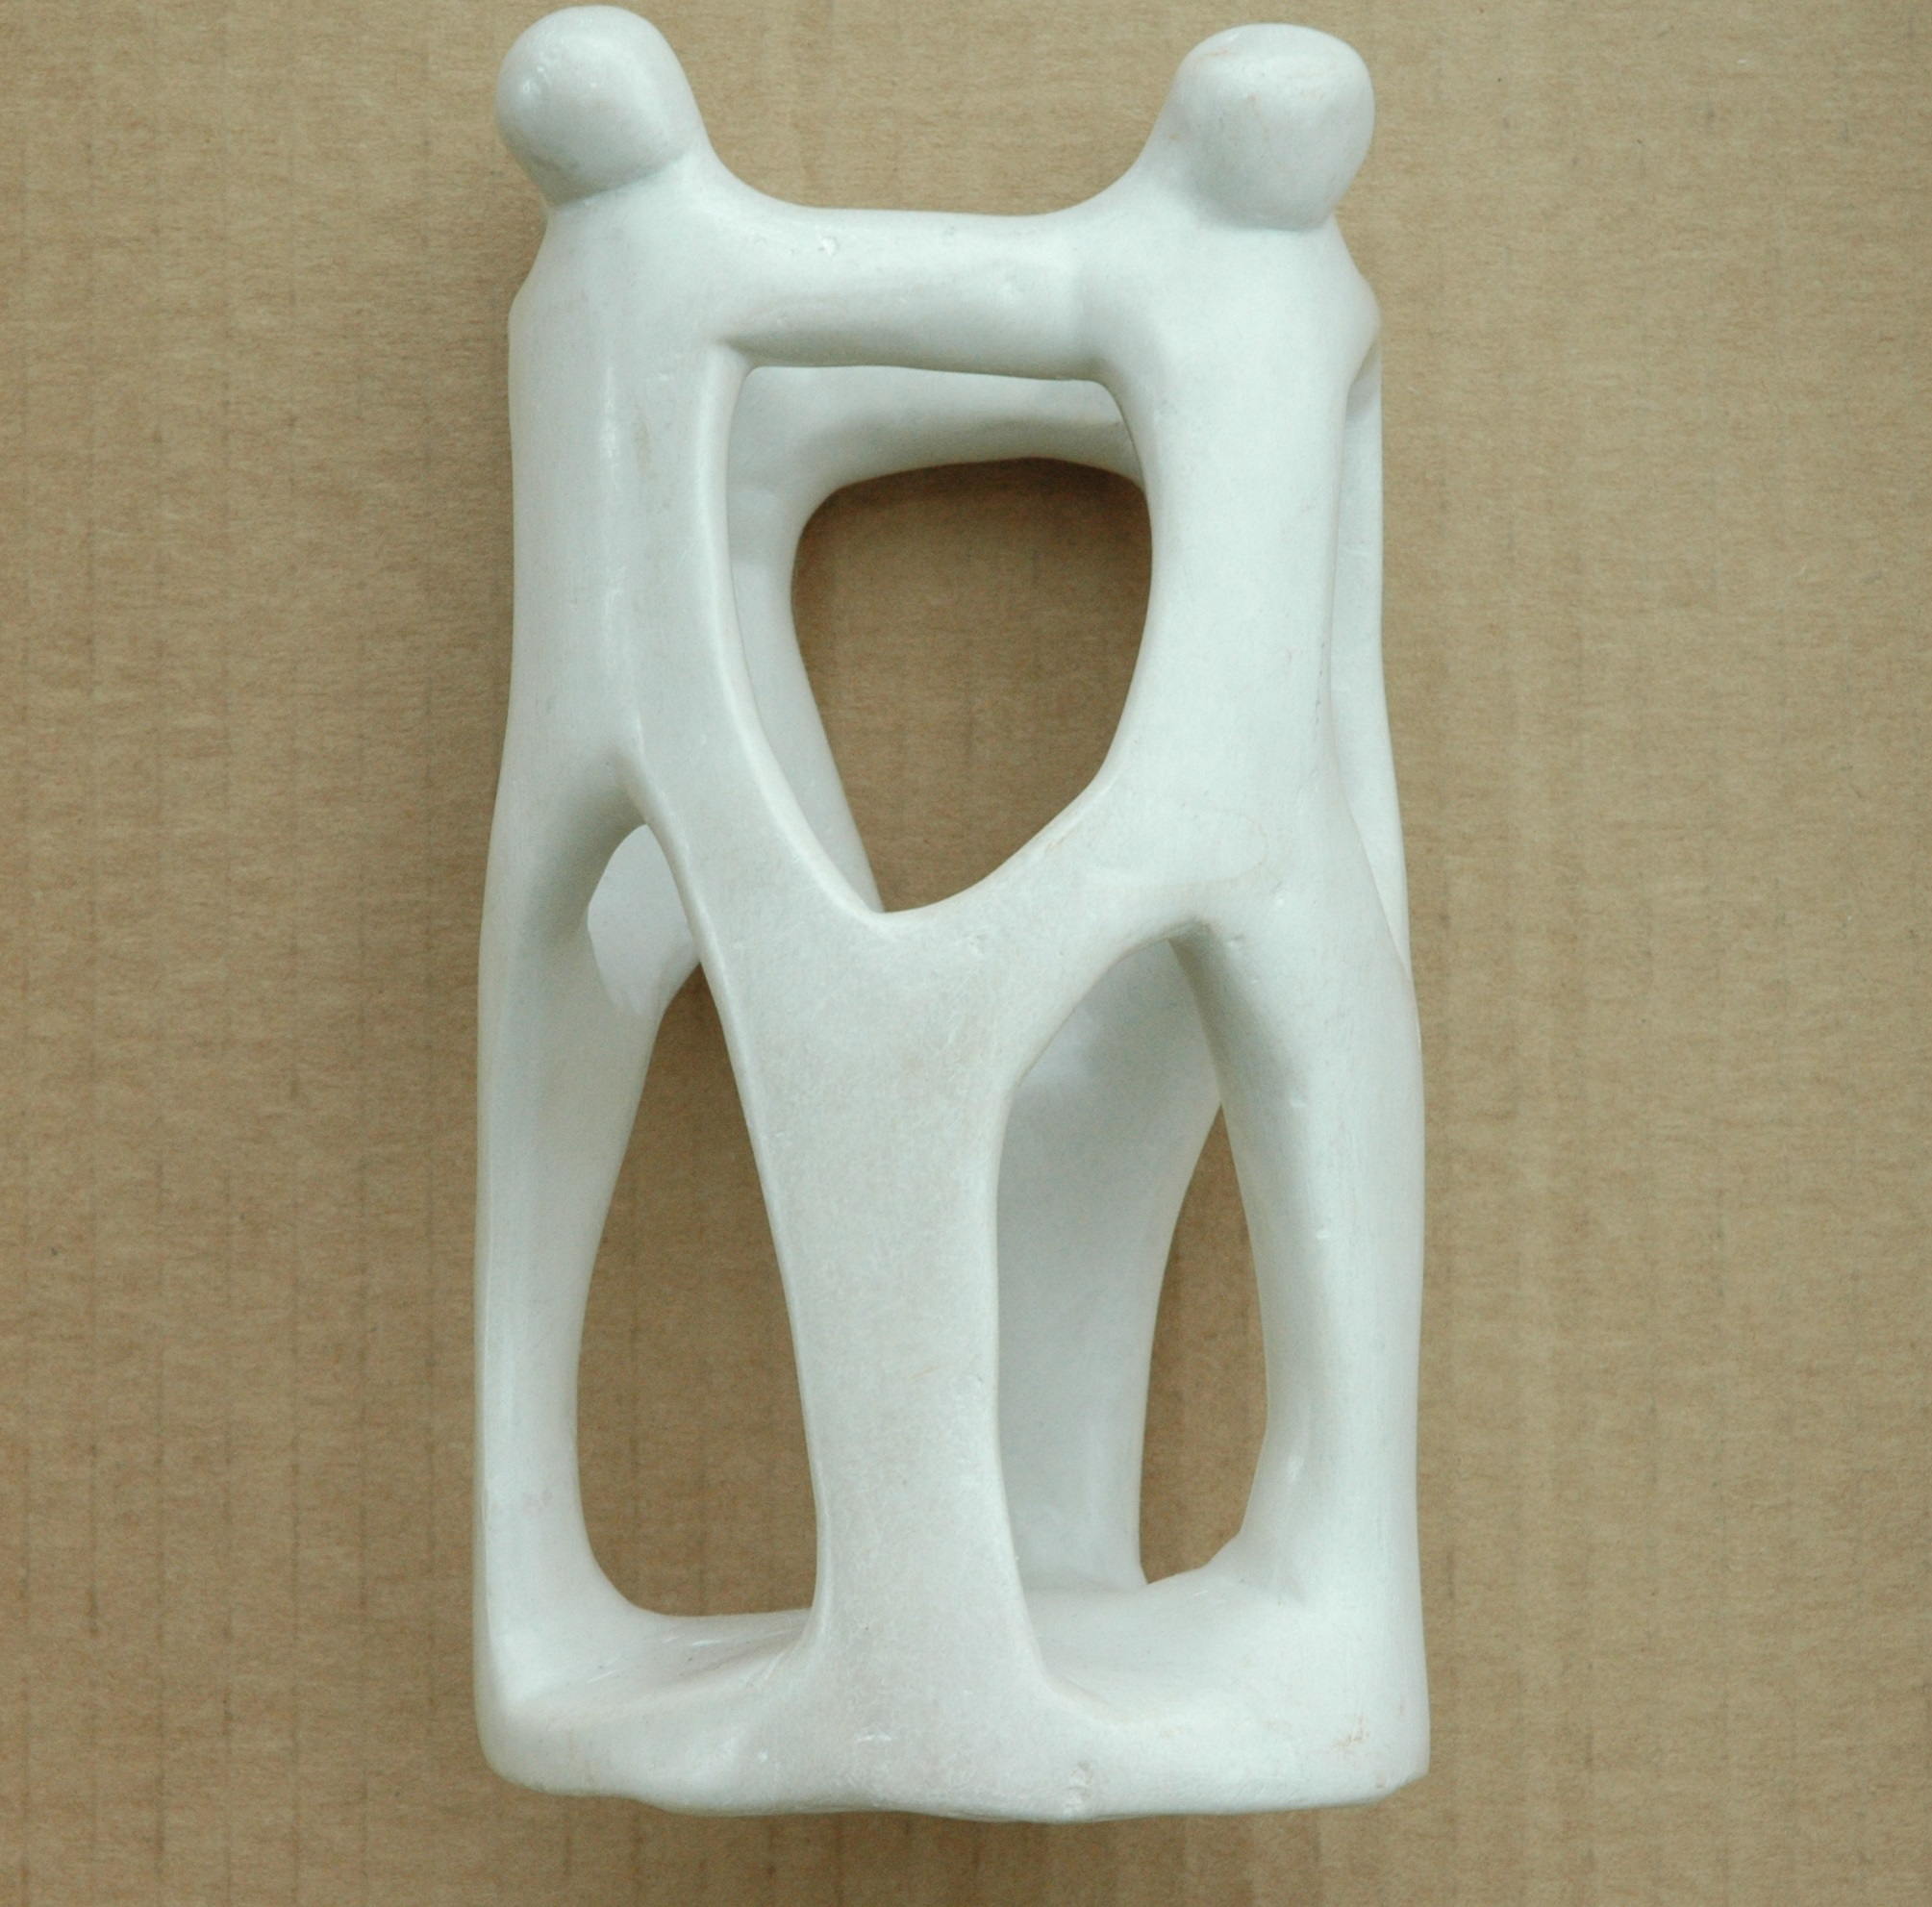
\includegraphics[width=0.33\textwidth]{interp/real_world_img/statue/statue}} &
  \multicolumn{3}{l}{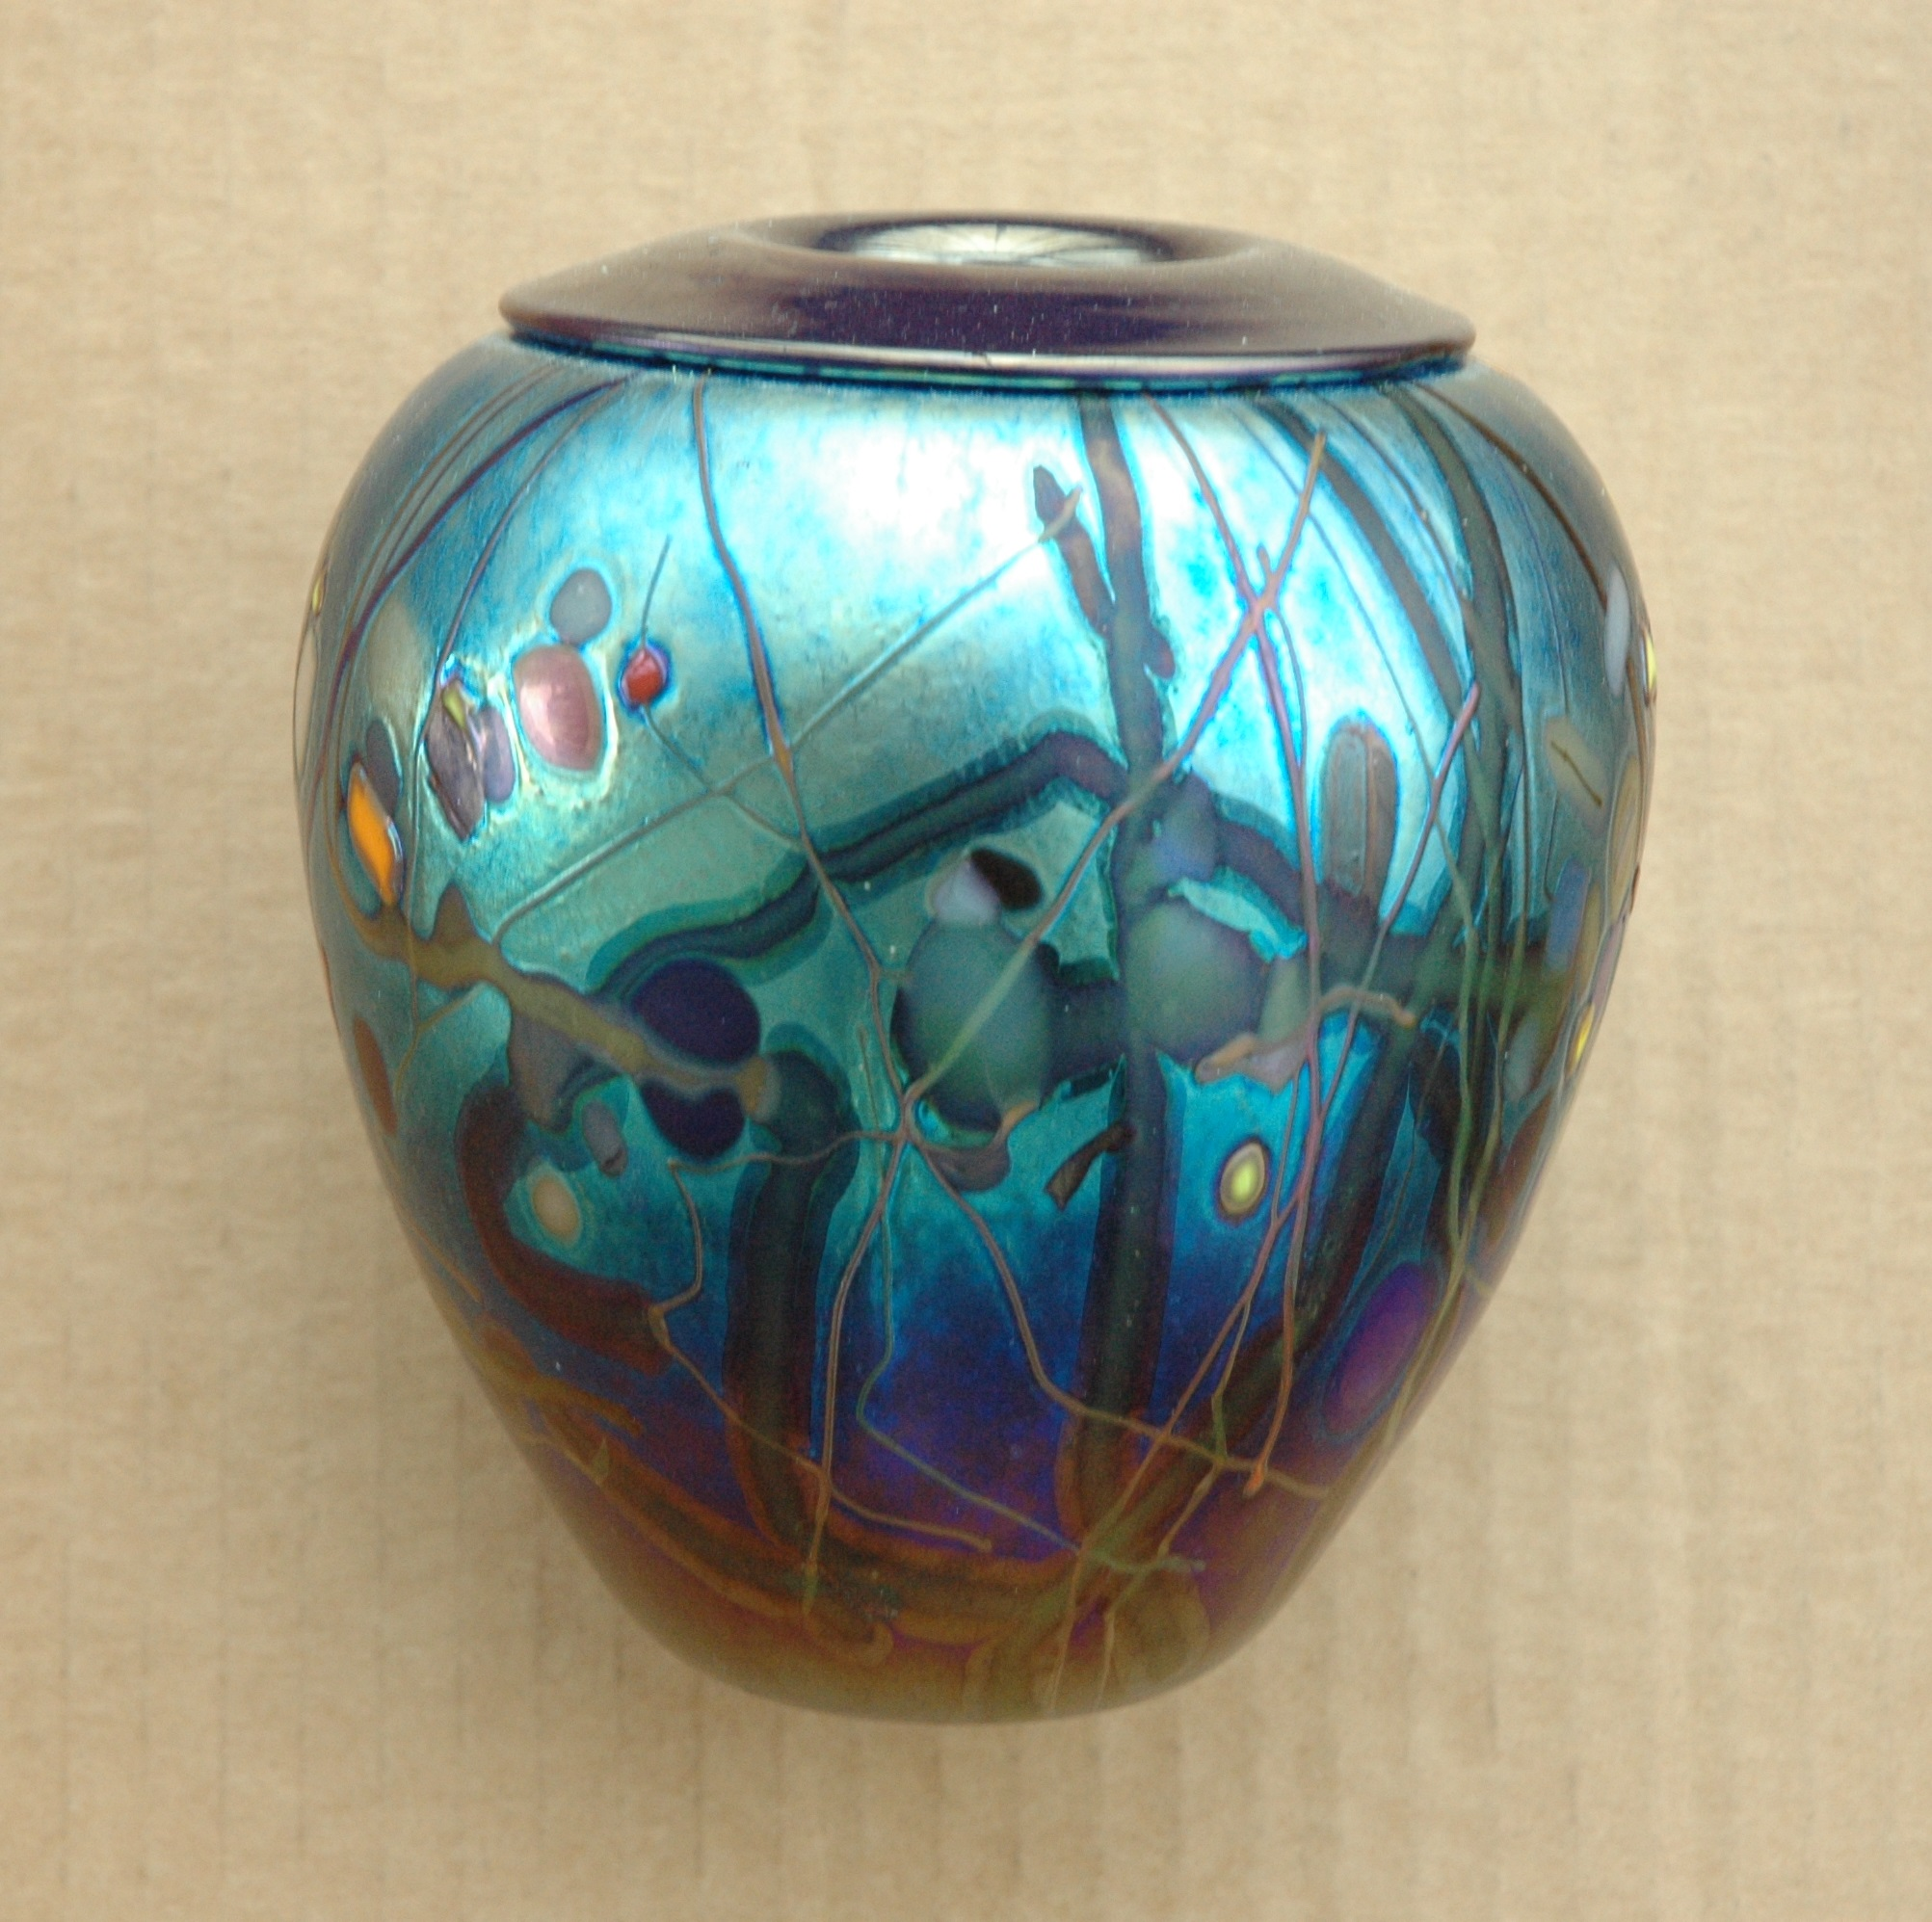
\includegraphics[width=0.33\textwidth]{interp/real_world_img/vase/vase}}\\
  % \includegraphics[width=0.1\textwidth]{interp/real_world_img/pot/base_00} &
  % \includegraphics[width=0.1\textwidth]{interp/real_world_img/pot/base_01} & &
  % \includegraphics[width=0.1\textwidth]{interp/real_world_img/statue/base_00} & & &
  % \includegraphics[width=0.1\textwidth]{interp/real_world_img/vase/base_00} &
  % \includegraphics[width=0.1\textwidth]{interp/real_world_img/vase/base_01}\\
  \multicolumn{3}{c}{(g). pot} & \multicolumn{3}{c}{(h). statue} & \multicolumn{3}{c}{(i). vase} \\
  \end{tabular}
  \caption{Images of the real-world objects.}
  \label{fig:real_data_material}
\end{table}

\section{Parameters of real-world objects}
\begin{table}[!htbp]
  \centering
  \begin{tabular}{*{3}{p{8mm}}*{2}{p{15mm}}|r}
  \toprule
  % & & & & & \multicolumn{3}{c}{Metrics}\\
  Class & Texture & Albedo & Specularity & Roughness & Mapping\\
  \midrule
  box & 0.8 & 0.8 & 0.2 & 0.8 & PMVS, EPS, GSL\\
  cat0 & 0.5 & 0.5 & 0.2 & 0.2 & PMVS\\
  cat1 & 0.2 & 0.2 & 0.2 & 0.2 & None\\
  cup & 0.2 & 0.8 & 0.5 & 0.2 & EPS, GSL\\
  dino & 0.2 & 0.5, 0.8 & 0.2 & 0.8 & EPS, GSL\\
  house & 0.8 & 0.2, 0.8 & 0.2 & 0.2 & PMVS, GSL\\
  pot & 0.8 & 0.2, 0.5 & 0.2 & 0.2 & PMVS\\
  status & 0.2 & 0.8 & 0.2 & 0.8 & EPS, GSL\\
  vase & 0.8 & 0.2, 0.5 & 0.5 & 0.2 & PMVS\\
  \bottomrule
  \end{tabular}
  \caption{Property list for the real-world objects}
  \label{tab:real_data_prop_list}
\end{table}

\section{Results of real-world objects}
\begin{figure}[!htbp]
\centering
\begin{tabular}{l|cccc}
Mapping & PMVS & EPS & GSL & VH (BL)\\
\midrule
PMVS, EPS, GSL &
\fcolorbox{green}{white}{\raisebox{-.5\height}{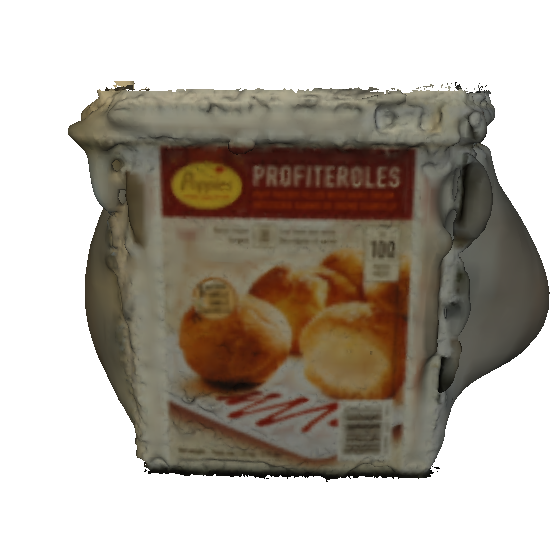
\includegraphics[width=0.2\textwidth]{interp/real_interp/box/box_mvs}}}&
\fcolorbox{green}{white}{\raisebox{-.5\height}{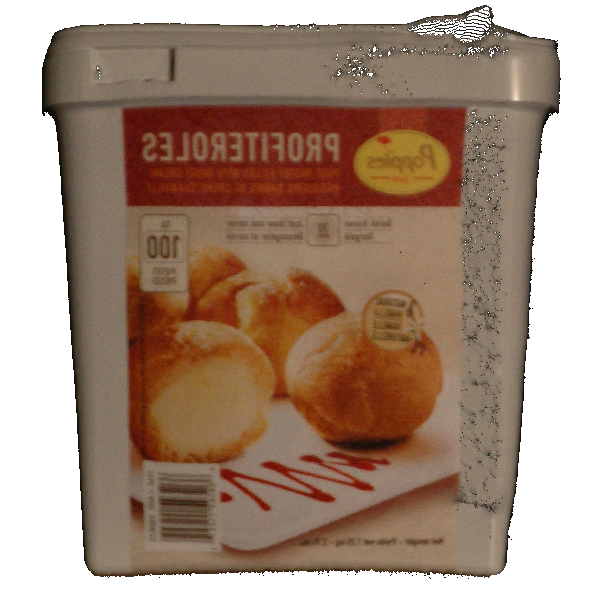
\includegraphics[width=0.2\textwidth]{interp/real_interp/box/box_ps}}}&
\fcolorbox{green}{white}{\raisebox{-.5\height}{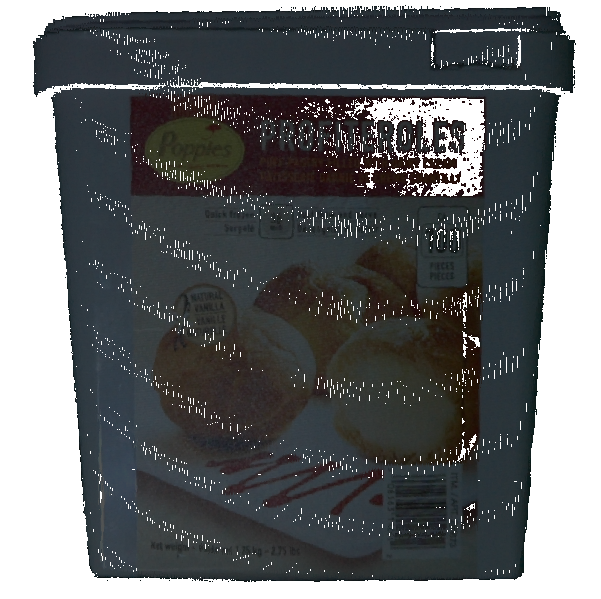
\includegraphics[width=0.2\textwidth]{interp/real_interp/box/box_sl}}}&
\raisebox{-.5\height}{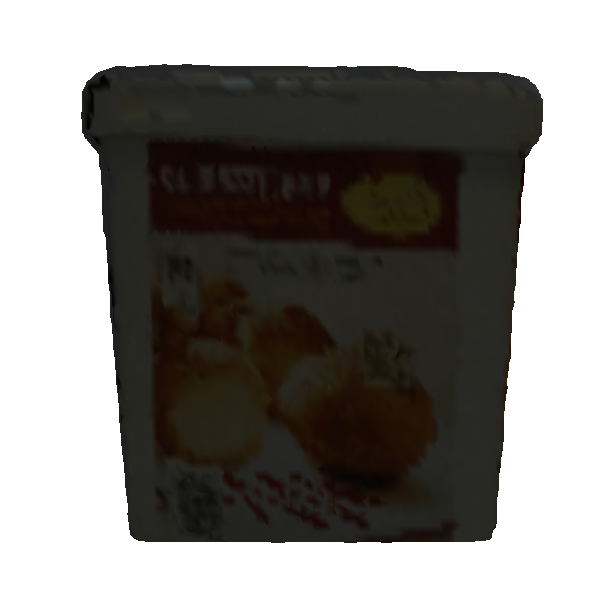
\includegraphics[width=0.2\textwidth]{interp/real_interp/box/box_sc}}\\
PMVS &
\fcolorbox{green}{white}{\raisebox{-.5\height}{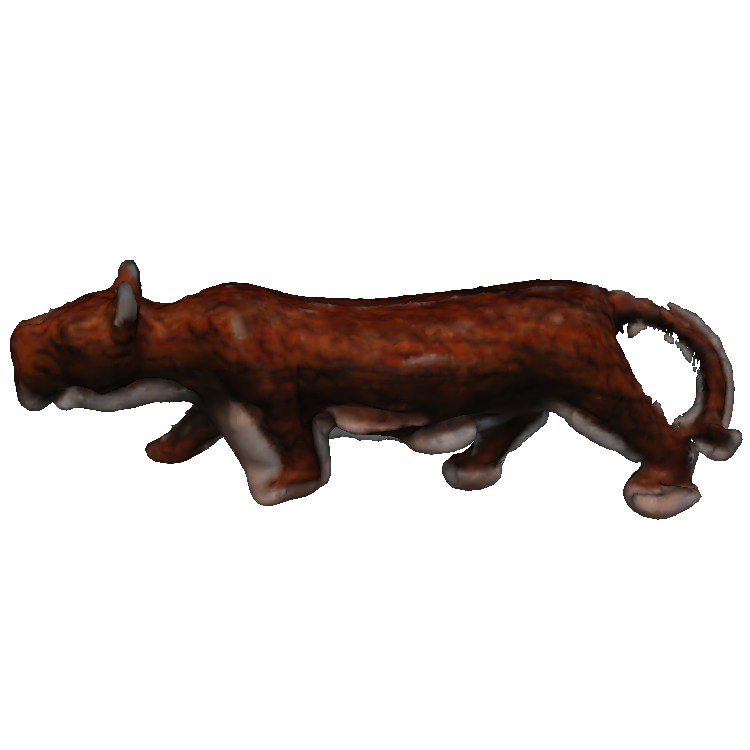
\includegraphics[width=0.2\textwidth]{interp/real_interp/cat0/cat0_mvs}}}&
\raisebox{-.5\height}{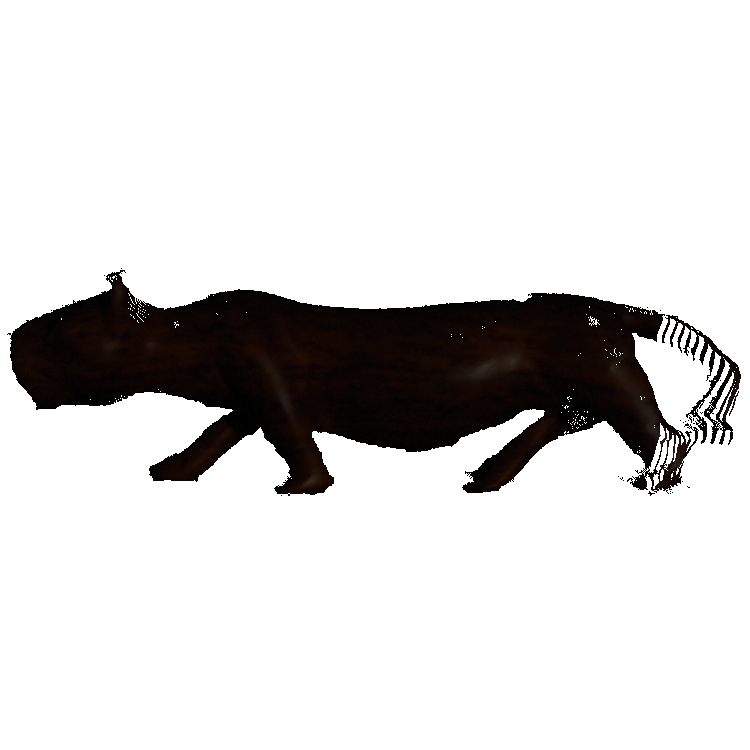
\includegraphics[width=0.2\textwidth]{interp/real_interp/cat0/cat0_ps}}&
\raisebox{-.5\height}{
\includegraphics[width=0.2\textwidth]{interp/real_interp/cat0/cat0_sl}}&
\raisebox{-.5\height}{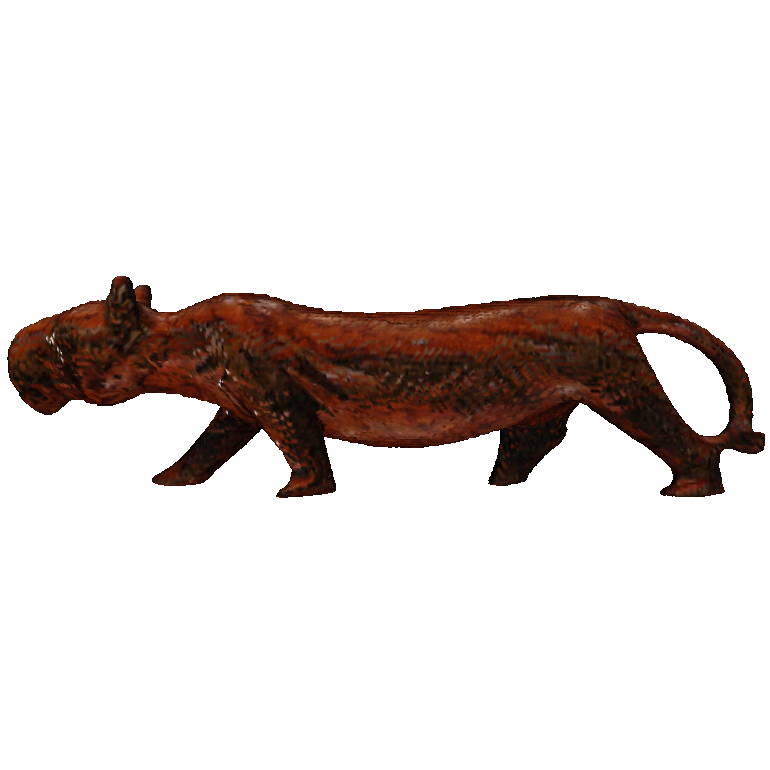
\includegraphics[width=0.2\textwidth]{interp/real_interp/cat0/cat0_sc}}\\
None &
\raisebox{-.5\height}{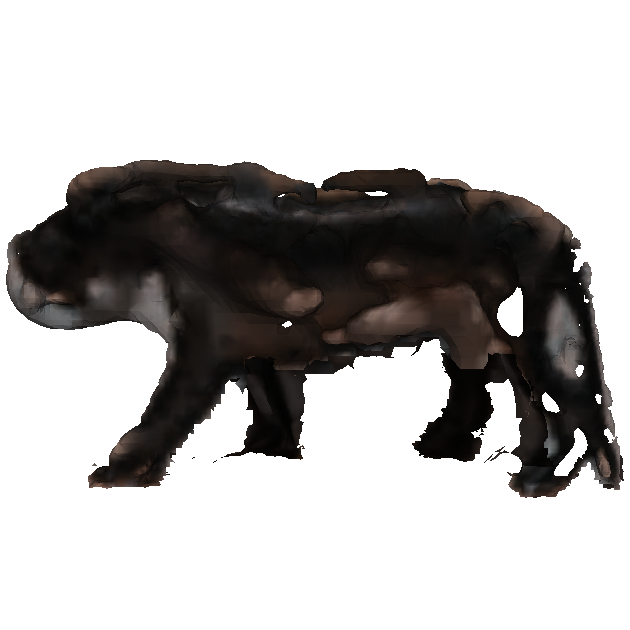
\includegraphics[width=0.2\textwidth]{interp/real_interp/cat1/cat1_mvs}}&
\raisebox{-.5\height}{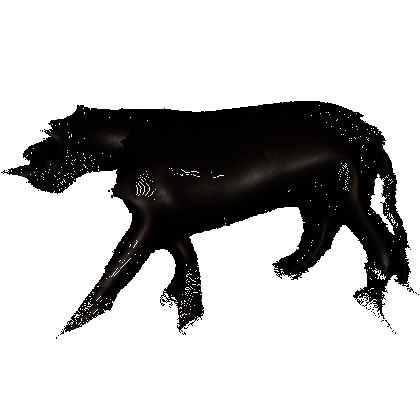
\includegraphics[width=0.2\textwidth]{interp/real_interp/cat1/cat1_ps}}&
\raisebox{-.5\height}{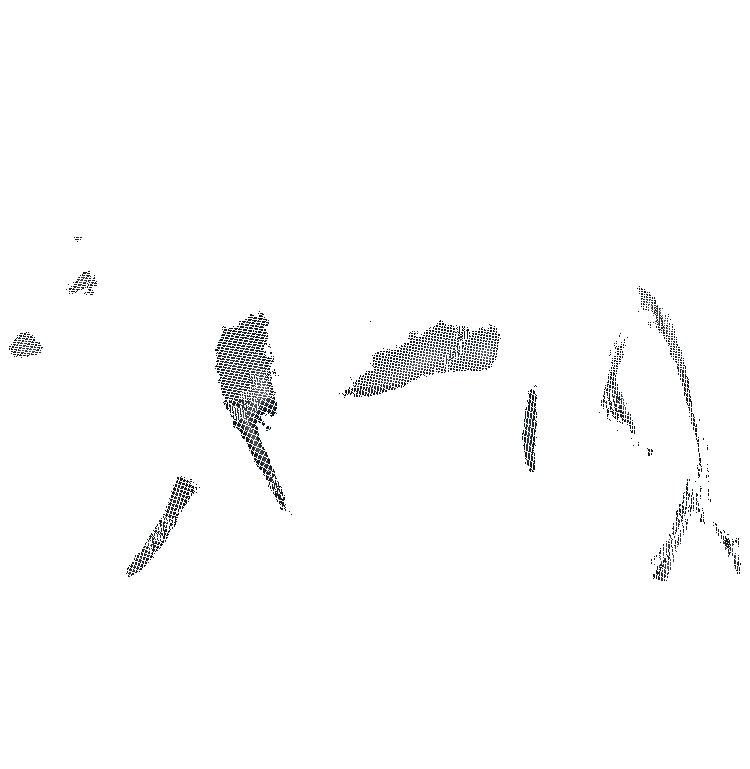
\includegraphics[width=0.2\textwidth]{interp/real_interp/cat1/cat1_sl}}&
\raisebox{-.5\height}{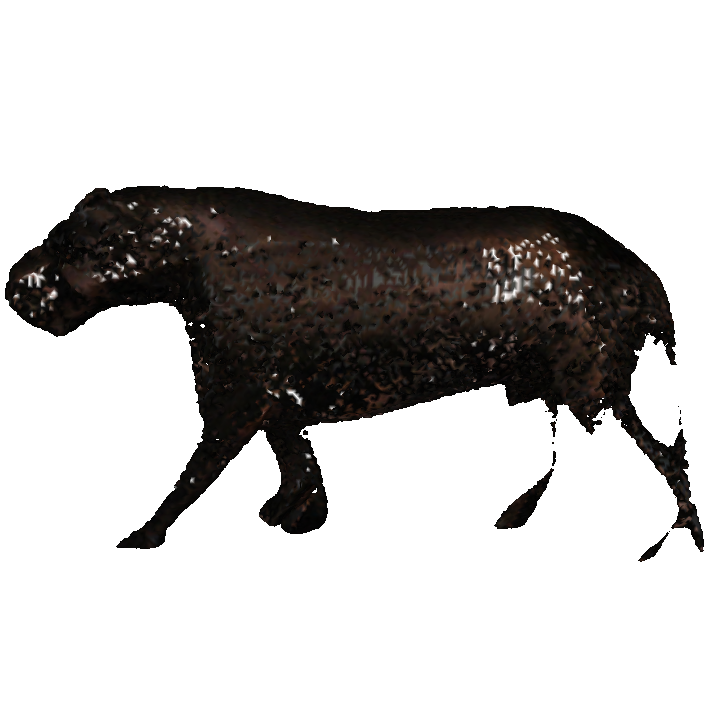
\includegraphics[width=0.2\textwidth]{interp/real_interp/cat1/cat1_sc}}\\
EPS, GSL &
\raisebox{-.5\height}{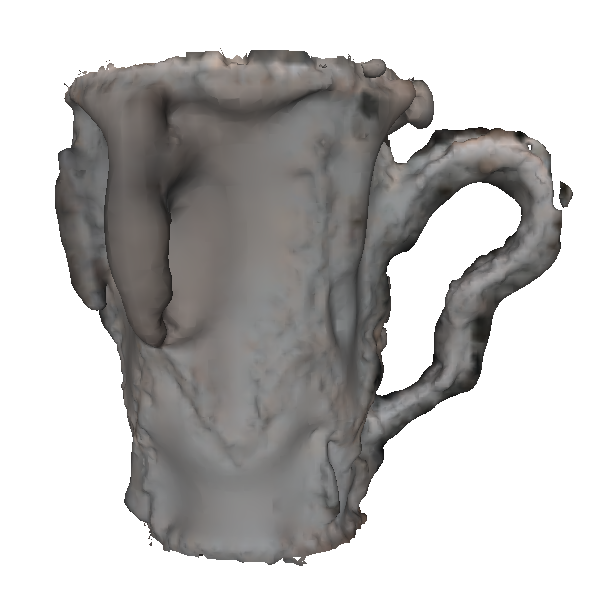
\includegraphics[width=0.2\textwidth]{interp/real_interp/cup/cup_mvs}}&
\fcolorbox{green}{white}{\raisebox{-.5\height}{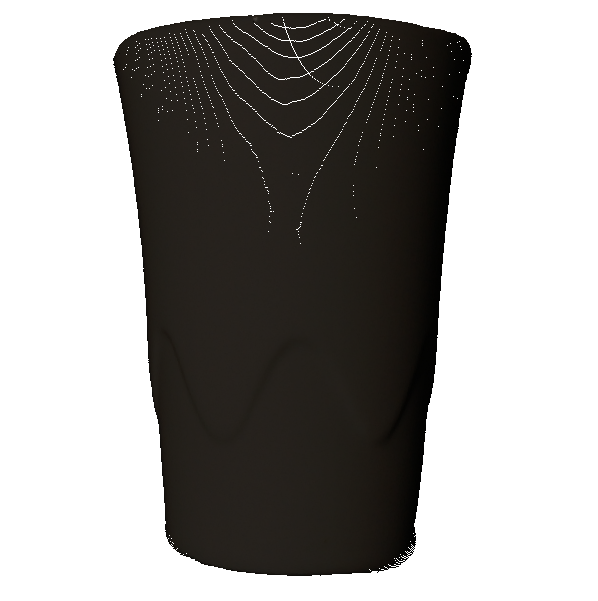
\includegraphics[width=0.2\textwidth]{interp/real_interp/cup/cup_ps}}}&
\fcolorbox{green}{white}{\raisebox{-.5\height}{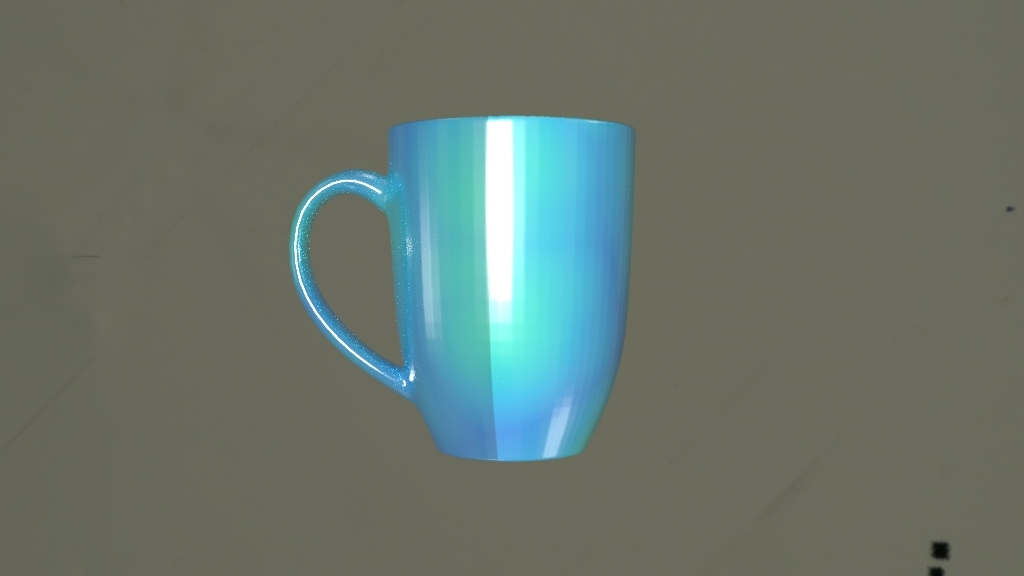
\includegraphics[width=0.2\textwidth]{interp/real_interp/cup/cup_sl}}}&
\raisebox{-.5\height}{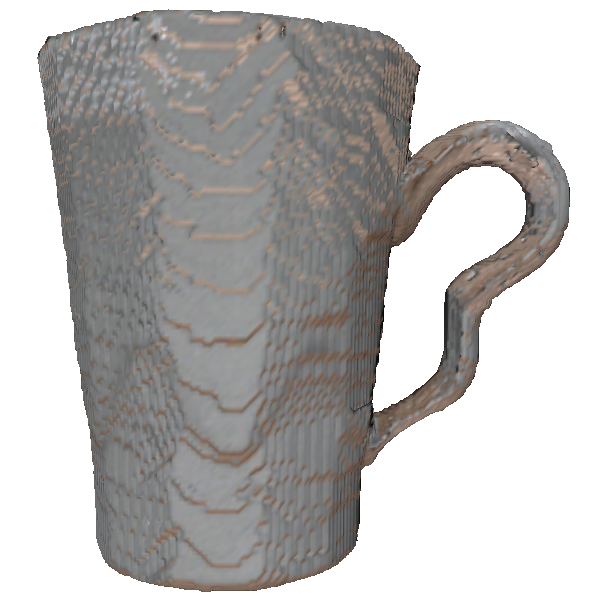
\includegraphics[width=0.2\textwidth]{interp/real_interp/cup/cup_sc}}\\
EPS, GSL &
\raisebox{-.5\height}{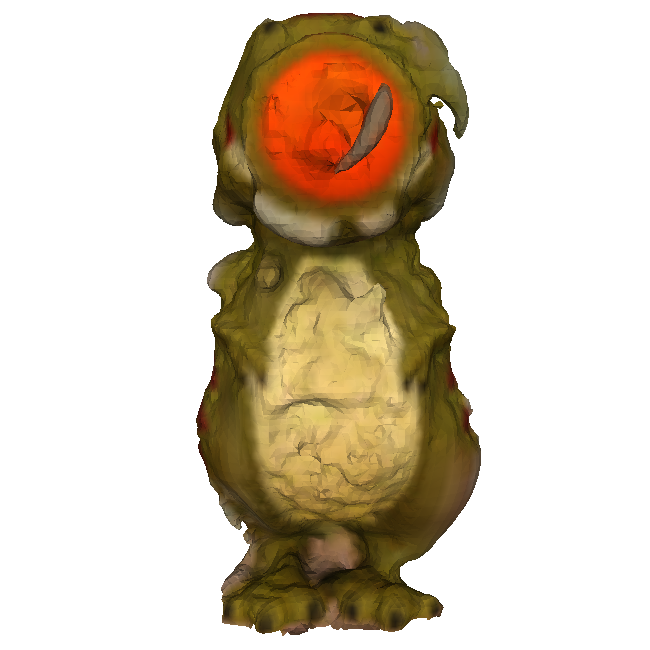
\includegraphics[width=0.2\textwidth]{interp/real_interp/dino/dino_mvs}}&
\fcolorbox{green}{white}{\raisebox{-.5\height}{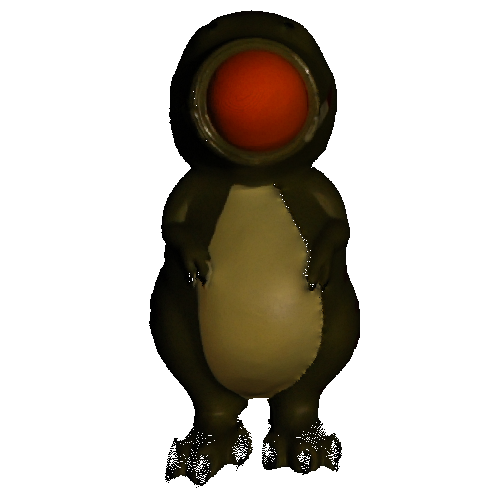
\includegraphics[width=0.2\textwidth]{interp/real_interp/dino/dino_ps}}}&
\fcolorbox{green}{white}{\raisebox{-.5\height}{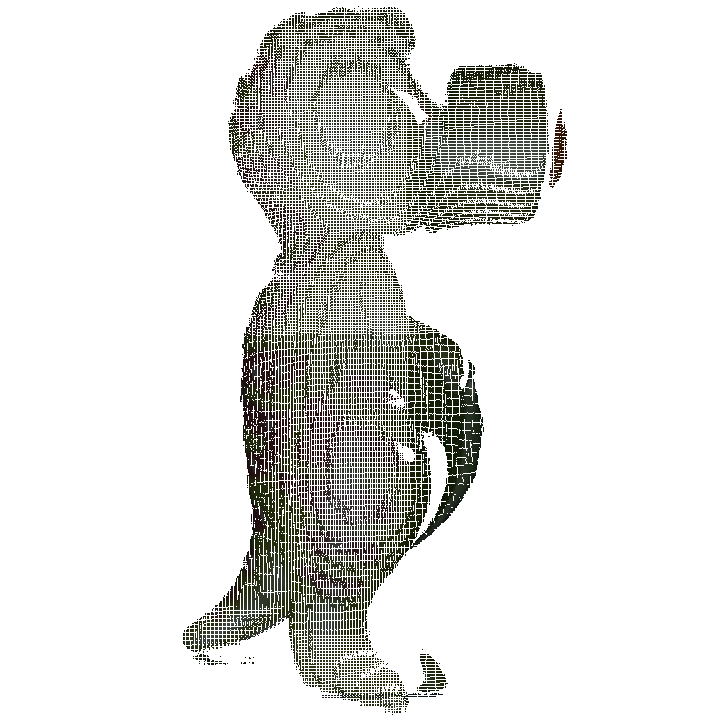
\includegraphics[width=0.2\textwidth]{interp/real_interp/dino/dino_sl}}}&
\raisebox{-.5\height}{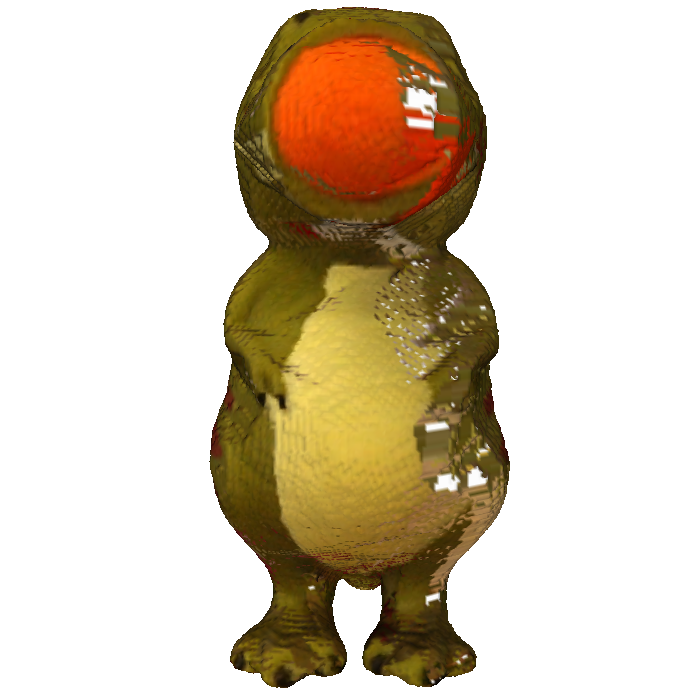
\includegraphics[width=0.2\textwidth]{interp/real_interp/dino/dino_sc}}\\
PMVS, GSL &
\fcolorbox{green}{white}{\raisebox{-.5\height}{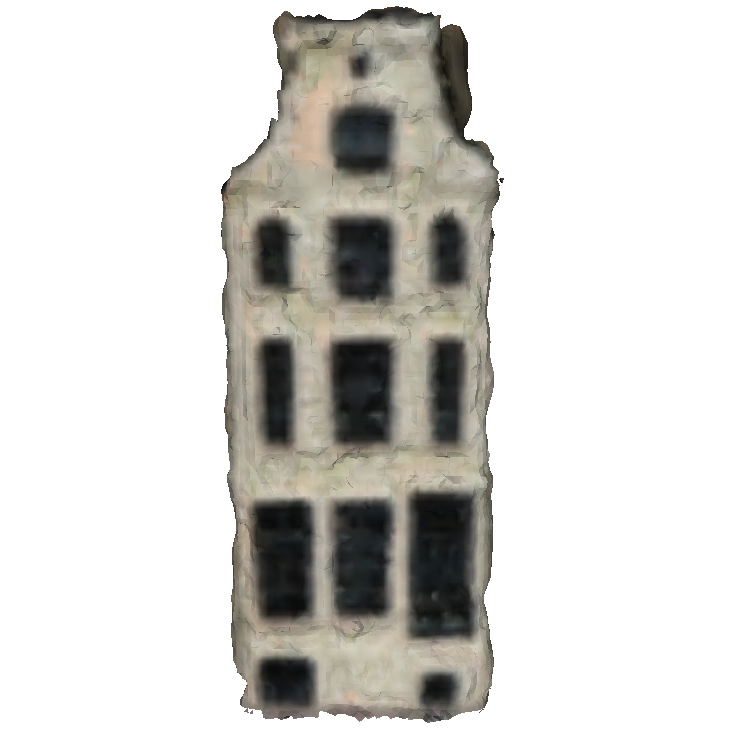
\includegraphics[width=0.2\textwidth]{interp/real_interp/house/house_mvs}}}&
\raisebox{-.5\height}{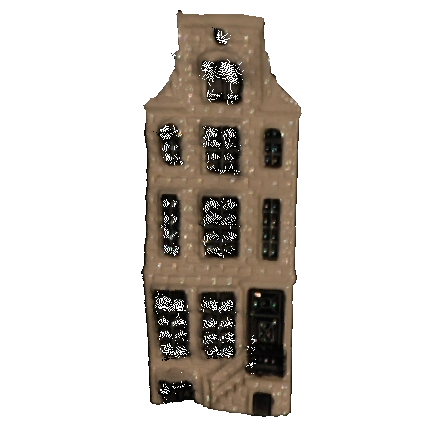
\includegraphics[width=0.2\textwidth]{interp/real_interp/house/house_ps}}&
\fcolorbox{green}{white}{\raisebox{-.5\height}{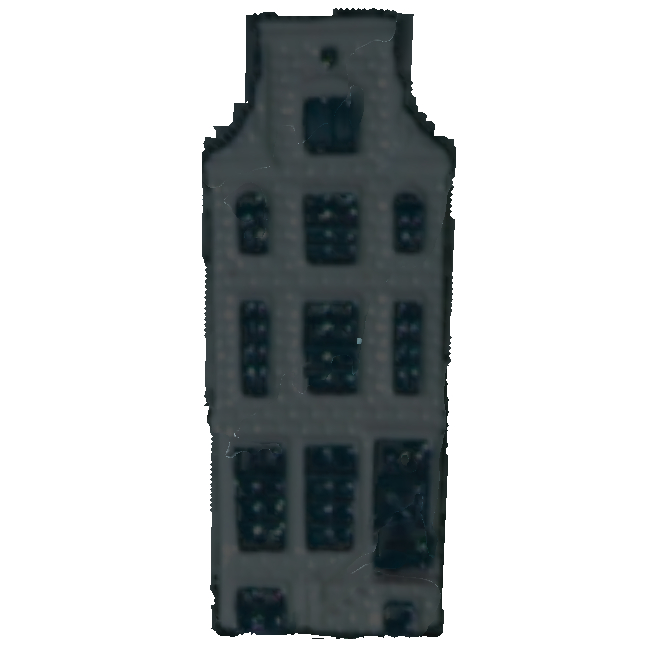
\includegraphics[width=0.2\textwidth]{interp/real_interp/house/house_sl}}}&
\raisebox{-.5\height}{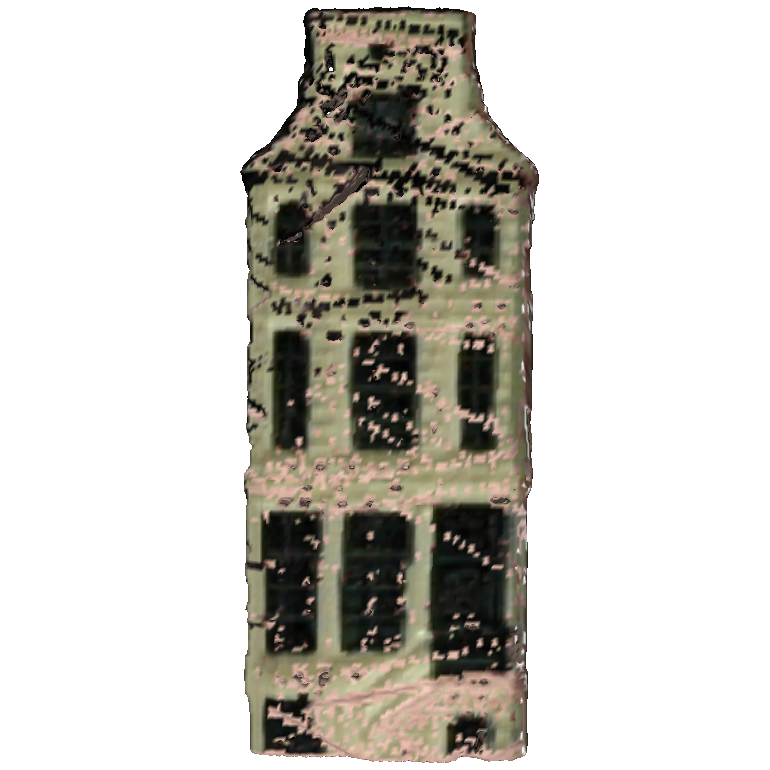
\includegraphics[width=0.2\textwidth]{interp/real_interp/house/house_sc}}\\
\bottomrule
\end{tabular}
\caption{Reconstruction results of MVS, PS, SL, and the baseline method VH.}
\label{fig:test_real_world_img}
\end{figure}

\begin{figure}[h!]
\centering
\begin{tabular}{l|cccc}
Mapping & PMVS & Example-based PS & Gray SL & VH(BL)\\
\midrule
PMVS &
\fcolorbox{green}{white}{\raisebox{-.5\height}{\includegraphics[width=0.2\textwidth]{interp/real_interp/pot/pot_mvs}}}&
\raisebox{-.5\height}{\includegraphics[width=0.2\textwidth]{interp/real_interp/pot/pot_ps}}&
\raisebox{-.5\height}{\includegraphics[width=0.2\textwidth]{interp/real_interp/pot/pot_sl}}&
\raisebox{-.5\height}{\includegraphics[width=0.2\textwidth]{interp/real_interp/pot/pot_sc}}\\
EPS, GSL &
\raisebox{-.5\height}{\includegraphics[width=0.2\textwidth]{interp/real_interp/statue/statue_mvs}}&
\fcolorbox{green}{white}{\raisebox{-.5\height}{\includegraphics[width=0.2\textwidth]{interp/real_interp/statue/statue_ps}}}&
\fcolorbox{green}{white}{\raisebox{-.5\height}{\includegraphics[width=0.2\textwidth]{interp/real_interp/statue/statue_sl}}}&
\raisebox{-.5\height}{\includegraphics[width=0.2\textwidth]{interp/real_interp/statue/statue_sc}}\\
PMVS &
\fcolorbox{green}{white}{\raisebox{-.5\height}{\includegraphics[width=0.2\textwidth]{interp/real_interp/vase/vase_mvs}}}&
\raisebox{-.5\height}{\includegraphics[width=0.2\textwidth]{interp/real_interp/vase/vase_ps}}&
\raisebox{-.5\height}{\includegraphics[width=0.2\textwidth]{interp/real_interp/vase/vase_sl}}&
\raisebox{-.5\height}{\includegraphics[width=0.2\textwidth]{interp/real_interp/vase/vase_sc}}\\
\bottomrule
\end{tabular}
\caption{Reconstruction results of MVS, PS, SL, and the baseline method VH (cont'd).}
\label{fig:test_real_world_img}
\end{figure}